\documentclass[11pt,a4paper]{report}

% Aberstwyth MMP Project Report Template for LaTeX
%
% Authors: Neil Taylor (nst@aber.ac.uk) and Dr. Hannah Dee (hmd1@aber.ac.uk) 
%
% This has been adapted from the Leeds Thesis template and the 
% Group Project template for Computer Science in Aberystywth University.
% 
% All comments and suggestions welcome.
%
% Template designed to be used with pdflatex: it may need alteration to
% run with a different LaTeX engine.
%
% Note - this is offered as a starting point for your work. You are not 
% required to use this template and can choose to create your own document 
% without it.

% This template is suitable for students with an engineering-style project, 
% which will be most students in the department. If your project is a research-oriented 
% project, look at the alternative template.

% To build document on the unix command line, run four commands:
 
% pdflatex mmp-report
% bibtex mmp-report
% pdflatex mmp-report
% pdflatex mmp-report

% you will end up with mmp-report.pdf. Before submitting, add your user ID as a prefix, 
% e.g. abc01-mmp-report.pdf 
\usepackage{StylesAndReferences/mmp-report}

% the following packages are used for citations - You only need to include one. 
%
% Use the cite package if you are using the numeric style (e.g. IEEEannot). 
% Use the natbib package if you are using the author-date style (e.g. authordate2annot). 
% Only use one of these and comment out or remove the other one. 
\usepackage{cite}
%\usepackage{natbib}

%%%% Title and Section Colours %%%%
% Modify these values to change the colours used for title, sections and subsections.
% Each value is a range of 0-255 in RGB colourspace.
% Idea courtesy of discussion at 
% https://www.overleaf.com/learn/latex/Using_colours_in_LaTeX
% and
% https://tex.stackexchange.com/questions/75667/change-colour-on-chapter-section-headings-lyx
% 
% If you prefer to have black headers, then comment out the following lines
\definecolor{mmpTitle}{RGB}{10, 85, 145}
\definecolor{mmpSection}{RGB}{10,85,155}
\definecolor{mmpSubsection}{RGB}{79,129,189}

\chapterfont{\color{mmpTitle}}  % sets colour of chapters
\sectionfont{\color{mmpSection}}  % sets colour of sections 
\subsectionfont{\color{mmpSubsection}} % sets colour subsections
\subsubsectionfont{\color{mmpSubsection}} % sets colour subsections

%%%% end of Title and Section Colours %%%%


%%%% Report Type %%%%
%% comment/uncomment depending on the type of report you want to generate
%\reporttype{Engineering}
\reporttype{Research}
%%%% end of Report Type %%%%


\begin{document}

%TC:ignore

% all of the include directives below refer to tex files
% so %TC:ignore 

\title{Group-based Ant Colony Optimisation for Solving TSPs}

% Your name
\author{Charlie Robinson}

% Your email 
\authoremail{chr40@aber.ac.uk}

\degreeschemecode{G401} %e.g. G400 
\degreeschemetitle{Computer Science with Integrated Year in Industry} % e.g. Computer Science
\degreetype{BSc}

\modulecode{CS39440} % i.e. CS39440, CC39440, CS39620
\moduletitle{Major Project} % i.e. Major Project or Minor Project

\date{10th May 2020} % i.e. the date of the current version of your report

\status{Release} % Use draft until you create the release version. Then, change this to Release.
\version{1.0}

% The title and name of your supervisor.
\supervisor{Dr. Richard Jensen} 

%The email for your supervisor. 
\supervisoremail{rkj@aber.ac.uk}

\maketitle

%TC:endignore
 includes cover.tex - to change the content,
% edit the tex file

\pagenumbering{roman}

% This is the front page
%TC:ignore 

\title{Group-based Ant Colony Optimisation for Solving TSPs}

% Your name
\author{Charlie Robinson}

% Your email 
\authoremail{chr40@aber.ac.uk}

\degreeschemecode{G401} %e.g. G400 
\degreeschemetitle{Computer Science with Integrated Year in Industry} % e.g. Computer Science
\degreetype{BSc}

\modulecode{CS39440} % i.e. CS39440, CC39440, CS39620
\moduletitle{Major Project} % i.e. Major Project or Minor Project

\date{10th May 2020} % i.e. the date of the current version of your report

\status{Release} % Use draft until you create the release version. Then, change this to Release.
\version{1.0}

% The title and name of your supervisor.
\supervisor{Dr. Richard Jensen} 

%The email for your supervisor. 
\supervisoremail{rkj@aber.ac.uk}

\maketitle

%TC:endignore
                        

% Set up page numbering
\pagestyle{empty}

% declarations of originality 
\thispagestyle{empty}

%TC:ignore

%%%
%%% You must sign the declaration of originality. 
%%%
%%% You are submitting this electronically. Therefore, to sign, you 
%%% type your name and date to replace the .... characters. 
%%%
\section*{\centering Declaration of originality}

I confirm that:

\begin{itemize}
\item{This submission is my own work, except where 
clearly indicated.}

\item{I understand that there are severe penalties for Unacceptable Academic Practice, which can lead to loss of marks or even the withholding of a degree.}
 
\item{I have read the regulations on Unacceptable Academic Practice from the University's Academic Registry (AR) and the relevant sections of the current Student Handbook of the Department of Computer Science.}
 
\item{In submitting this work I understand and agree to abide by the University's regulations governing these issues.}
\end{itemize}

\vspace{2em}
Name Charlie Robinson  \\

\vspace{1em}
Date 10th May 2020\\

%%% 
%%% We would like to make a selection of final reports available to students that take 
%%% this module in future years. To enable us to do this, we require your consent. You 
%%% are not required that you do this, but if you do give your consent, then we will have 
%%% the option to select yours as one of a number of reports as examples for other 
%%% students. If you would like to give your consent, then please include the following 
%%% text and type your name and date to replace the .... characters. 
%%% 
%%% If you do not wish to give your consent, please remove this from your report. 
%%%
\vspace{1em}
\section*{\centering Consent to share this work}

By including my name below, I hereby agree to this project's report and technical work being made available to other students and academic staff of the Aberystwyth Computer Science Department.  

\vspace{2em}
Name ............................................................  \\

\vspace{1em}
Date ............................................................ \\

%TC:endignore

               

\thispagestyle{empty}

%TC:ignore

\section*{\centering Acknowledgements}


I am grateful to...

I'd like to thank...

%TC:endignore % Acknowledgements

\thispagestyle{empty}

%TC:ignore

\section*{\centering Abstract}

Include an abstract for your project. This should be approximately 300 words. 

The abstract is an overview of the work you have done. Highlight the purpose of the work and the key outcomes of the work.

%TC:endignore                 % Abstract

\pagenumbering{roman}
\pagestyle{fancy}
\fancyhead{}
\fancyfoot[C]{\thepage}
\renewcommand{\headrulewidth}{0 pt}
\renewcommand{\chaptermark}[1]{\markboth{#1}{}}

\tableofcontents   
\newpage
\listoffigures % comment out this line if you don't have any figures / graphics
\newpage 
\listoftables % comment out this line if you don't have any tables
\newpage

% Set up page numbering
\pagenumbering{arabic}

\setchapterheaderfooter

%TC:endignore

% include the chapters
\chapter{Background \& Objectives}

\section{Problem Description}

The Travelling Salesperson Problem (TSP) is tasked with solving the problem "Given a list of cities and the distances between each city what is the shortest possible route that visits each city once and then returns to the origin city". This shortest route is called a Hamiltonian Cycle and has many applications such as in the fields of logistics, route planning and manufacturing\cite{acobook}. Dantzig, Fulkerson and Johnson were the first people to attempt to solve TSPs through the use of branch and bound\cite{dantzig1954solution}, the time taken to solve TSPs through this method was too high to be practical so since then TSPs have attempted to be solved through the use of many new intuitive algorithms.

Every method to solve TSPs has a limit on the size of problems that it can solve because it would simply take too long to solve problems above a given size. My project is a way of solving TSPs through the use of clustering and an Ant Colony Optimisation (ACO) Algorithm.

There are many freely available data sets of TSPs I have used the ones provided by The University of Waterloo\cite{tsp_test_data_2009} these are all of varying sizes and complexity and are provided in the common TSPLIB95 format, they also all have their optimal solutions noted so that easy comparisons can be made and so I can see how my algorithm performs. This TSP data is split into two main categories National (World) and VLSI, world test data is based on cities on a map and range in size from 29 nodes to 71,000 nodes, VSLI data is based on solder points in circuit boards. These two types of problems look very different and will require different types of clustering algorithms to properly solve. Figure \ref{fig:vlsi_tsp_data} shows VLSI test data and figure \ref{fig:world_tsp_data} shows an example of a world TSP problem.

\begin{figure}
    \centering
    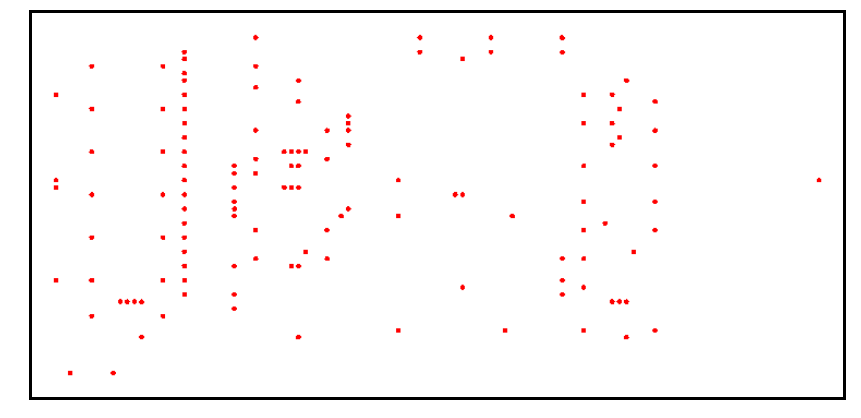
\includegraphics[width=\textwidth]{figures/vlsi_xqf131_tsp_data.png}
    \caption{Figure showing VLSI TSP test data, the nodes in this problem form in lines and therefore the clusters will need to extend and form into lines in order to get the most optimal soution. This problem came from \cite{xqf131_tsp_instance}.}
    \label{fig:vlsi_tsp_data}
\end{figure}

\begin{figure}
    \centering
    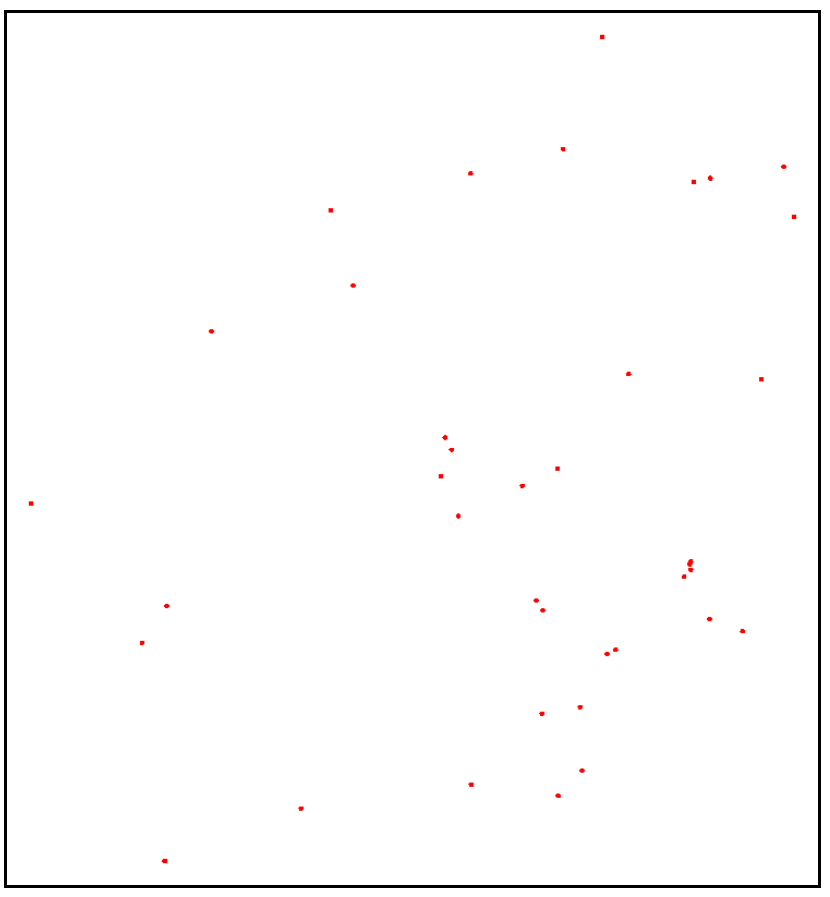
\includegraphics[width=\textwidth]{figures/world_dj38_tsp_data.png}
    \caption{Figure showing world TSP test data, the nodes form like cities on a map. This example is based on 38 cities from Djibouti. This problem came from \cite{dj38_tsp_instance}.}
    \label{fig:world_tsp_data}
\end{figure}

\section{Background}
My motivation for this project was based around my interest in Algorithms and finding new approaches to solve challenging problems, In 1991 ACO was first applied to solve TSPs\cite{dorigo1991distributed} this algorithm was called "Ant System" and was tested on several TSPs. It was able to solve TSPs of small sizes but didn't perform as well in solving larger problems. 

ACO is a probabilistic search technique which is used to find good paths through graphs. In the real world when an Ant leaves its nest to find food it initially randomly wanders, whilst it is wondering it is laying down a pheromone trail. When it finds some food it will follow its pheromone trail back to the nest but still has a chance to go off randomly. Ants aren't guaranteed to follow a trail of pheromone they can go off and randomly wonder, this is what allows the ants to find better paths between the food and their nests. ACO is based on this pheromone communication, figure \ref{fig:aco_pheremone_example} shows how an ants trail changes based on this pheromone. Over time this pheromone trail evaporates which reduces its attractiveness towards ants, the longer the path the more time it has to evaporate. A short path that gets travelled frequently will have much less evaporation because of the more ants travelling over it. This evaporation is also what leads to the ants avoiding a locally optimal solution because without it then the first path that was travelled would be the final path.

\begin{figure}
    \centering
    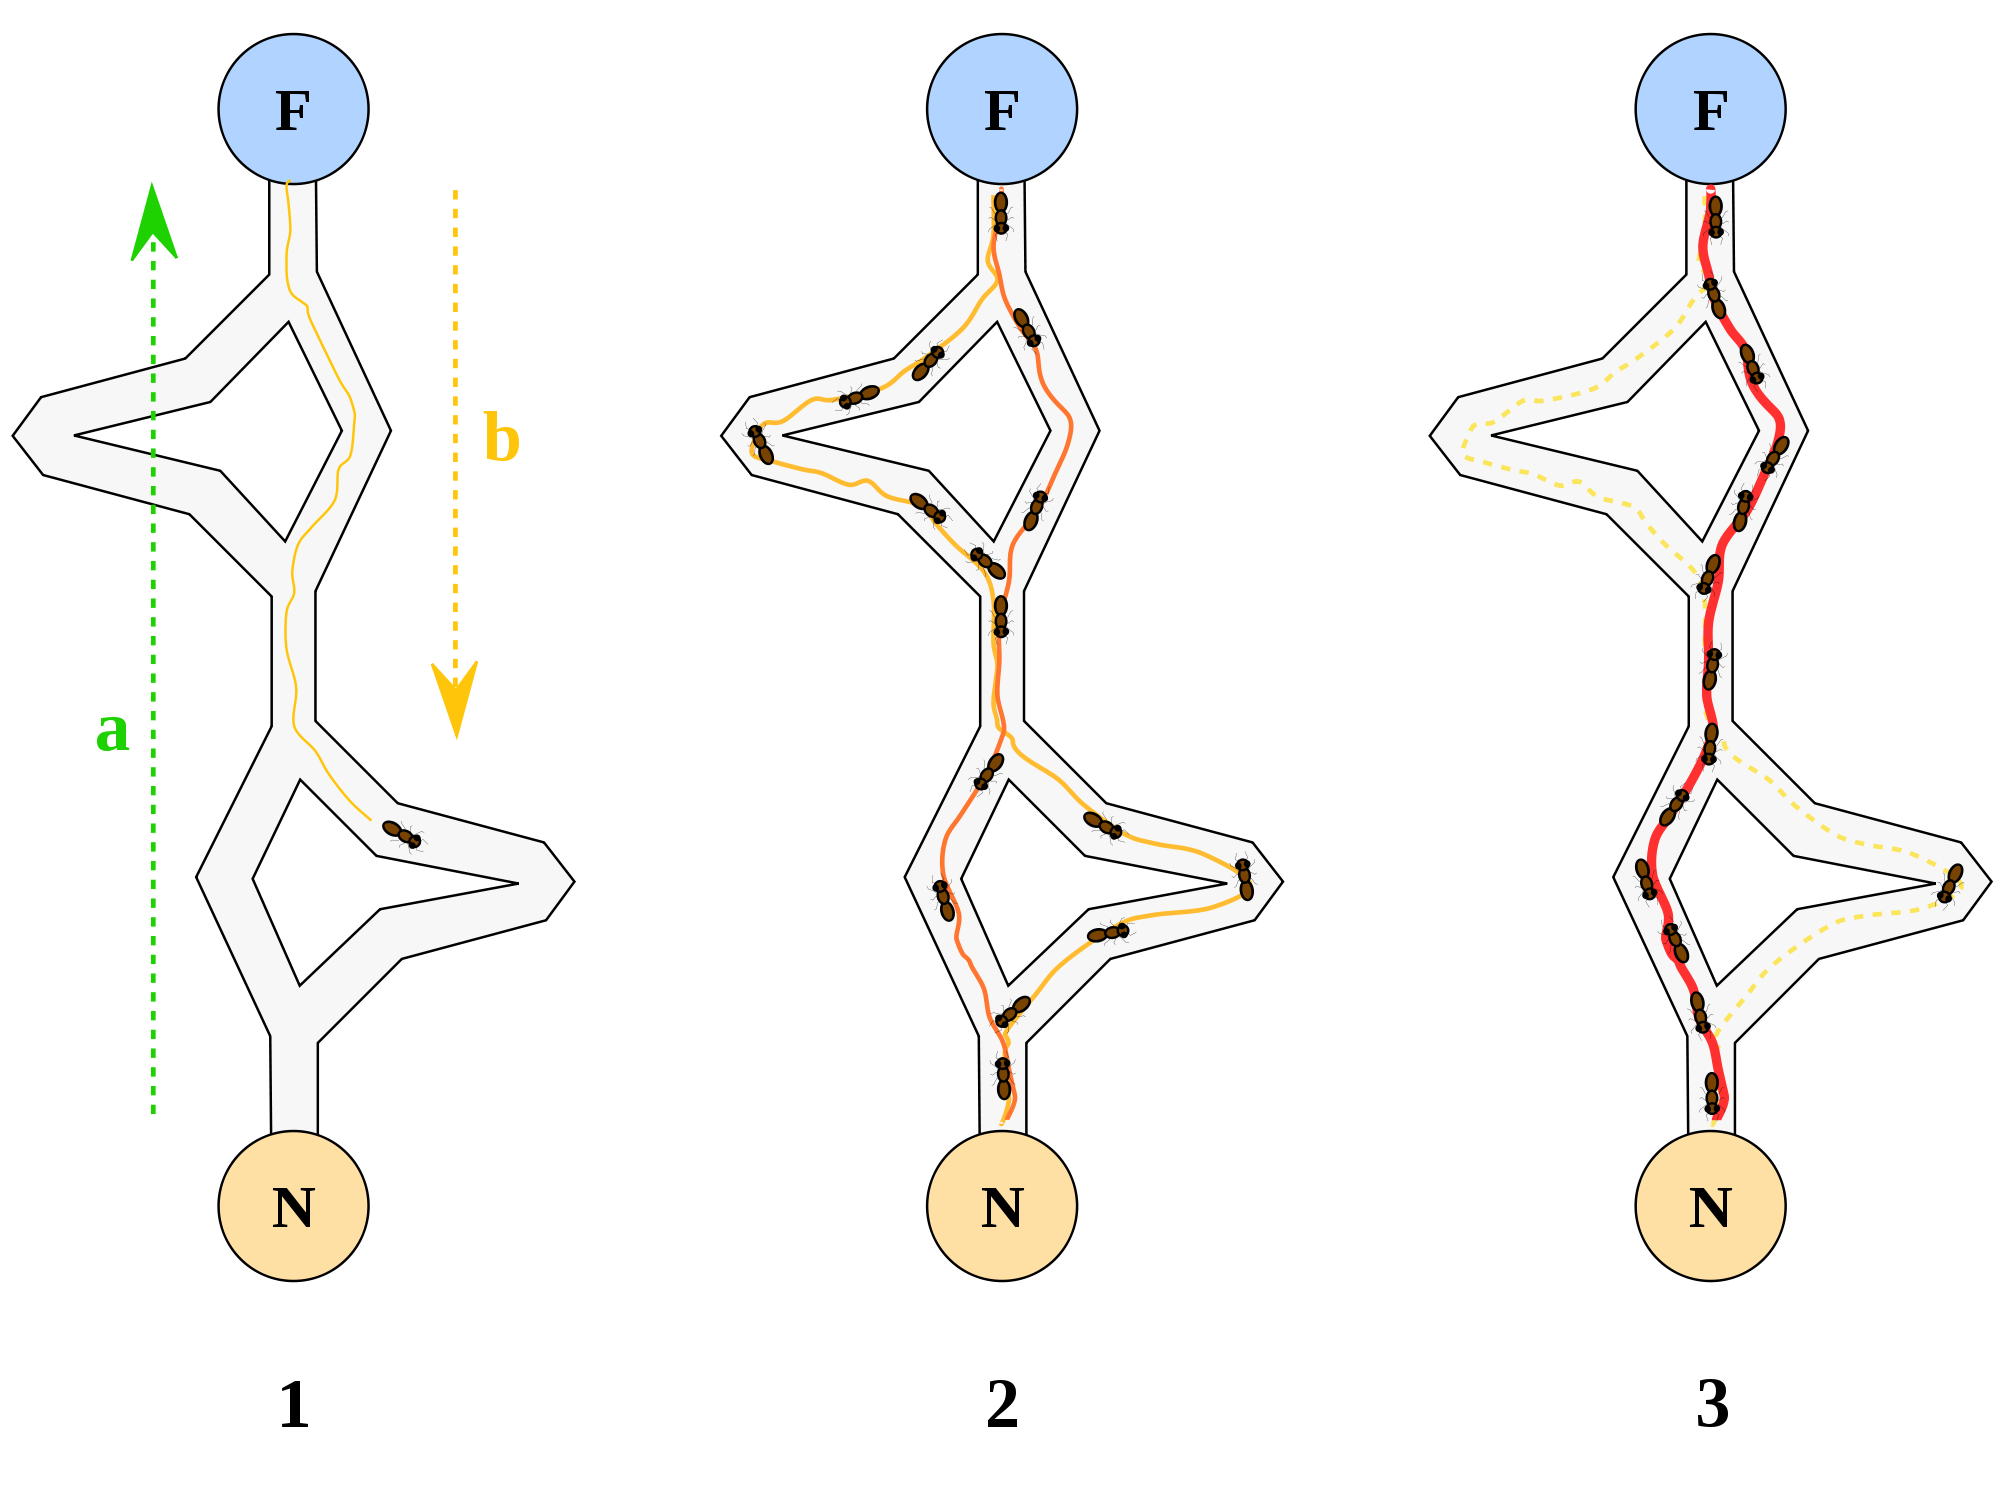
\includegraphics[width=\textwidth]{figures/aco_pheremone_demo.png}
    \caption{Figure showing how in nature ants deposit pheromone and change their paths based on the pheromone from other ants. The Ants choose a path based on the pheromone that has been deposited but there is also a random chance that the ant will choose a different route, this is what allows ACO to change routes and find a better solution.}
    \label{fig:aco_pheremone_example}
\end{figure}

There are a few key formulas that enable ACO to achieve this, the edge selection equation shown in figure \ref{eq:ACOEdgeselection} and the pheromone update equation which is shown in figure \ref{eq:pheremoneupdate}. 

\begin{figure}[h]
    \centering
    $
    p_{xy}^k =
    \frac
    { (\tau_{xy}^{\alpha}) (\eta_{xy}^{\beta}) }
    { \sum_{z\in \mathrm{allowed}_x} (\tau_{xz}^{\alpha}) (\eta_{xz}^{\beta}) }$
    \caption{This is the edge selection formula for ACO. Ant $k$ moves from state $x$ to state $y$ with this probability. $\tau_{xy}$ is the amount of pheromone deposited when transitioning from $x$ to $y$. $\alpha$ is a value equal to or greater than 0 which controls $\tau_{xy}$. $\eta_{xy}$ is how desirable that transition is, $\beta$ controls this desirability.}
    \label{eq:ACOEdgeselection}
\end{figure}

\begin{figure}[h]
    \centering
    $ \tau_{xy} \leftarrow
    (1-\rho)\tau_{xy} + \sum_{k}\Delta \tau^{k}_{xy}$
    
    $\Delta \tau^{k}_{xy} =
    \begin{cases}
    Q/L_k & \mbox{if ant }k\mbox{ uses curve }xy\mbox{ in its tour} \\
    0 & \mbox{otherwise}
    \end{cases}$
    \caption{This is the pheromone update equation. Pheromones are updated when an Ant completes its tour, the pheromones levels are increased for 'good' tours and decreased for 'bad' tours. $\tau_{xy}$ is the amount of pheromones deposited when transitioning from state $x$ to state $y$. $\rho$ is the pheromone evaporation constant, $\Delta \tau^{k}_{xy}$ is the amount of pheromone deposited by ant $k$. $Q$ is the pheromone constant value and $L_k$ is the tour length for ant $k$.}
    \label{eq:pheremoneupdate}
\end{figure}

ACO has several parameters you can tune; the number of iterations that it runs, the number of ants that are simulated, the amount of pheromone that is deposited, the amount of pheromone that evaporates each iteration, the weighting that the pheromone has on the ants decision, called the alpha value, and the weighting that the distance of the edge has on the ants decision, this is called the beta value. ACO algorithms make a choice between whether they will follow the pheromone deposits or change path and follow a heuristic, this is what the alpha and beta values are for. This allows the algorithm to be probabilistic and improve upon its tours, however because of this probabilistic nature it can produce different tours on consecutive runs. If you have a high alpha value then the ant is more likely to follow the other ants that came before it, and if you have a high beta value then the ant is more likely to choose a route that has the lowest distance. There is a balance to be struck because going to the closest node does not always result in the best overall tour.

ACO is not efficient at finding the solution for large problems because its run time is to high, it's possible to tune the parameters of the algorithm such as reducing the number of iterations it will perform however doing this could mean that it finds a worse solution. 

The main way to cut the run time of ACO is to cut down on the number of nodes. The run time of ACO is \[O(t\textsubscript{max}MN^2)\] where t\textsubscript{max} is the number of iterations, M is the number of ants and N is the number of nodes\cite{pang_chao-yang_ben-qiong_zhang_jie_wei_shan_zheng-chao_2014}. The run time is proportional to N\textsuperscript{2} so the only way to cut down the run time of the algorithm without compromising the quality of the solution is to cut down the number of nodes.

There are many different clustering algorithms available it is my goal to implement quite a few of them so that there is a choice and the different clustering algorithms can be analysed in respect to their effect on ACO. The Python library Scikit Learn\cite{scikit_learn_python_library} has implemented many different clustering algorithms\cite{scikit_clustering} and so I will be using that to do my clustering, I will choose a selection of these algorithms and should be able to compare them to see which ones perform better against ACO.

The tour that ACO produces may not be optimal because it didn't run for long enough or the parameters where not tuned correctly to fix this there is a local search algorithm called 2-opt that takes a tour created from a heuristic and attempts to improve it\cite{venhuis_2019} It improves the tour by reordering the nodes, it performs very well at removing paths in the tour that cross over each other but does not always find the optimal solution because it is bound to the tour that was found in the heuristic and simply finds the local optimum of this. 2-opt swaps two nodes to see if this improves the tour, there are other algorithms that act similarly 2.5-opt and 3-opt. These swap more nodes which can find bigger improvements.

When traversing the clustered tour there will need to be a way of going from the global clustered tour to the local inside each cluster tour. To do this there will need to be nodes assigned on each cluster that are the entry and exit nodes and then a tour will have to be made in each cluster from the entry node to the exit node. To find this tour I will implement ways of finding the solution with ACO and through a greedy nearest neighbours approach.

\section{Analysis}

\subsection{The Current State of Solving TSPs with ACO and Clustering}
As I've previously mentioned ACO has been applied to TSP many times before but this has mostly centred around using just ACO, in \cite{assesmentdiffacofortsp} different ACO algorithms are all put to work solving a particular TSP and assessed based on how quickly they take to run and how close to optimal their solution is. This paper considers five different ACO algorithms and offers a good comparison of how well suited these algorithms are to solve TSPs as well as offering good explanations of the types of ACO algorithms. 

Clustering has been used before as part of a solution to solve TSPs in \cite{clustering_with_local_search_heuristic}, in this study Clustering was used alongside a Genetic Algorithm and it showed that when clustering the data and then running the GA an improved TSP tour was found.

As briefly mentioned earlier \cite{pang_chao-yang_ben-qiong_zhang_jie_wei_shan_zheng-chao_2014} used ACO and clustering to solve TSPs and in their research they found that using clustering did speed up the ACO process they also created their own clustering algorithm the "Local Clustering Algorithm" which better expands to fit TSP data. 

The paper \cite{yang_shi_marchese_liang_2008} talks about using ACO to solve TSPs by dividing the nodes into groups and then visiting those groups. This is similar to clustering. It also uses mutation to avoid being locked into poor decisions allow the path to break out of a local minimum. It also uses 2-opt to speed up the finding of a good solution.

In \cite{10.1007/11839088_31} they create a new clustering algorithm which uses the features of ACO to group data. Existing clustering solutions converge prematurely and end up finding a local minimum this algorithm attempted to mitigate that by sending ants out along their paths and building up pheromone trails, at each step of the ants trail it selects a node that doesn't belong to a cluster and adds it to one. The ants deposit pheromones on nodes and nodes that have more pheromone are more attractive to ants. When the ants select nodes they use a combination of this pheromone and a euclidean distance heuristic. 

\subsection{Intended Approach}
There are many directions to take this project and things that I could discuss and do however because I've only got a few months to do this project I'm going to be limited. I would like to mostly look at the interactions of ACO on solving TSPs and seeing how clustering affects this.

I had to decide on the clustering algorithms that I wanted to use, as I mentioned briefly before I am using the Python library Scikit Learn to do my clustering and this implements 10 clustering algorithms. I want to choose clustering algorithms that all work in slightly different ways so that I have a better chance to find a clustering algorithm that better works for TSP data. I have selected the K-Means, Affinity Propagation, DBSCAN, OPTICS and Birch clustering algorithms. 

The K-Means algorithm splits the data up into N non-overlapping clusters each data point belongs to only one cluster, it attempts to place the clusters as far away from each other whilst also making the intra-cluster data points as similar as possible. K-means works well for a very large number of nodes and quite a lot of clusters. This algorithm is good to use because it allows the number of clusters to be specified. This particular implementation requires a parameter called 'n\_init', this value indicates the number of times the algorithm will be ran with different centroid the final result will be the run that has the best output in terms of the parameters mentioned above.

Affinity Propagation is different to the others because it works out the number of clusters there should be it does this by working out the similarities between each data point. It doesn't work very well with a large number of nodes this is because of the computation and memory resources needed to calculate the number of nodes. It requires two arguments max\_iterations and convergence\_iterations, Affinity Propagation runs in iterations and tries to converge points together into clusters. max\_iterations refers to the maximum number of iterations that will be run in total before it stops, convergence\_iterations is the number of iteration that need to happen sequentially with no change in order for the algorithm to stop. 

The next clustering algorithm I chose was DBSCAN, this chooses the number of clusters based on two values eps and min\_samples. A higher min\_samples value or a lower eps value means that a higher density is needed for a cluster to form. The min\_samples value refers to the number of nodes that need to be in a neighbourhood for that to be considered a core point and a cluster to form around it, the eps value refers to the maximum distance between two nodes for them to be considered in the same neighbourhood, it's not the maximum distance between points in a cluster if there is a dense but spread out cluster then the size of the cluster can be larger then this value. The eps value is the most important factor to choose correctly. This algorithm scales up to a large amount of nodes and quite a lot of cluster. This also supports classifying nodes as 'noise' these nodes do not fit into any cluster because they are too far away from other nodes.

I chose the OPTICS algorithm because like DBSCAN it supports classifying nodes as noise and it doesn't require the number of clusters to be set but unlike DBSCAN it doesn't require an eps value. It is very similar to DBSCAN in that it finds areas of high density but it differs in its approach to find the clusters because it generates a reach ability graph this allows it to find a sensible density value in order to build clusters. It is better suited to large datasets than DBSCAN however at the sizes that I will be examining I am unsure if this will matter. It requires a parameter called min\_samples this is the same as the parameter of the same name for DBSCAN, it affects the number of nodes that need to be together for the nodes to form into a neighbourhood.

The last clustering algorithm I chose was BIRCH, this algorithm works by building a tree for the data that you want to cluster. It requires three arguments; the branching factor, the number of clusters and a threshold value. This algorithm works well with a large number of clusters and a large number of nodes, this was the reason it was chosen.

In the time I have I will not be able to create an algorithm that can deal with massive TSPs that contain 10's of thousands of nodes or an algorithm that can necessarily find an optimal solution to every piece of data. I will instead focus on smaller problems and evaluating the results of these questions.

The questions that I propose for this project are;

\subsubsection{Does clustering allow ACO to be applied to larger problems.}

This question is about seeing how clustering impacts the run time of ACO and if clustering the data means that the run time is lower. To evaluate this question I will choose several pieces of TSP data of various sizes with both VLSI and world TSP data used, then I will have a run that does ACO only and a run that does ACO with a clustering algorithm. The run times and solution lengths will be calculated and compared. During these tests 2-opt will not be ran and the ACO parameters will stay the same for every test.

\subsubsection{To what effect do different clustering algorithms have on the quality and run time of the solution.}

This question is about seeing the change that clustering algorithms have on the solution. To run this experiment I will use the same ACO algorithm and parameters and then use different clustering algorithms to see if there is one that is particularly suited to use with TSP data. I will use TSP data of varying sizes as well as TSP that is of the VLSI type and the world type. To find the tour inside each cluster I will use both ACO and the greedy nearest neighbours approach. 

It would be interesting to see if I could create a new algorithm that can better deal with TSP data. In 'Applying Data Clustering Feature to Speed Up Ant Colony Optimization'\cite{pang_chao-yang_ben-qiong_zhang_jie_wei_shan_zheng-chao_2014} they create a new local clustering algorithm that measures the direction in which TSP data extends. This allows the clusters to better form around TSP data which should result in a better overall solution. It would be nice to implement my own clustering solution but I feel in the time I have that this may not necessarily be possible. It might be possible to improve existing clustering methods to better account for TSP data or speed up the process of clustering. 

The best kind of clustering algorithms to use will be ones that can deal with data that doesn't belong to any specific cluster, in most TSP problems there will be data that will not neatly fit into any specific cluster and this should be able to be dealt with. 

When it comes down to analysing the clustering algorithms that allow the number of clusters to be set I will vary the number of clusters.

\subsubsection{When using 2-opt with ACO and clustering what effect do the clusters have on the overall solution, does 2-opt end up finding the same solution or nearly the same solution regardless of the clustering algorithm used.}

This is about seeing how clustering really affects the final solution when 2-opt is used to smooth the solution out and find the local optimal solution, is this local optimum solution the same regardless of clustering algorithm used. This will also be able to show if there is a clustering algorithm that is superior for this application. To run this test I will keep the ACO algorithm and parameters the same and change the clustering algorithm. I will run this test on various sizes of TSP data on both world and VLSI data types. 

\subsubsection{What effect does varying the ACO parameters have on the solution.}

ACO can have a huge impact over the final solution, if the ACO run gave a bad solution then 2-opt can take longer and possibly not find as good a solution as it could of. ACO has a lot of parameters that can be tuned and it would be interesting to identifying the ones that most impact a TSP solution.

To run this experiment I would choose a world and VLSI TSP problem and a clustering algorithm. I would then vary the ACO parameters and see how these affected the quality of the solution found. I could measure this both before and after 2-opt has been ran to also see how ACO impacts the 2-opt run.
%\addcontentsline{toc}{chapter}{Development Process}
\chapter{Software Process}

I followed an Agile approach in my project because the requirements for my project evolved as I progressed, as I researched more and learnt more about the area I had more ideas about what I wanted to include and having an Agile approach allowed me to incorporate these ideas. 

At the start of my project I drew up a rough weekly plan that would guide me through the project and allow me to see how I was progressing overall, this can be seen in figure\ref{fig:initial_weekly_plan}. This plan was useful for me to start getting an overall idea of the scope of the project and allowed me to start to split the project up into separate sections.

For the first week I followed the Kanban process and used the online tool Glo Boards\cite{glo_board}, I however quickly realised that Kanban was not the right process to use because Kanban is generally about improving an already established process and as I was just starting I didn't have a process to improve so it didn't make a huge amount of sense to follow. 

I soon switched to using Scrum, this made a lot more sense because the project generally follows the design of a Scrum project already. I had sprints that lasted a week because each week I would have a meeting and you could consider this meeting to be a sort of extended stand-up, I discussed and demoed what I had worked on and we discussed what I could get done by next week. The product owner was me because I was ultimately in charge of the direction of the project and what new areas it would cover, my supervisor obviously had a guiding hand in what would be developed each week and what good progress would be.

When I switched to Scrum I realised that Glo Boards weren't really working for me so I switched to using Jira\cite{jira_site}. I made heavy use of epics to group my work and epics didn't work the way I wanted them to in Glo Boards. Jira was a tool that I used during my Industrial Year and I felt that it was very useful in planning and keeping track of work. I organised my work into epics and through the use of the backlog tool and the sprint management tool it was easy to see how well I was progressing and what still needed to be done. Figure \ref{fig:jira_epics} shows how Jira lays out epics in its road map view.

\begin{figure}
    \centering
    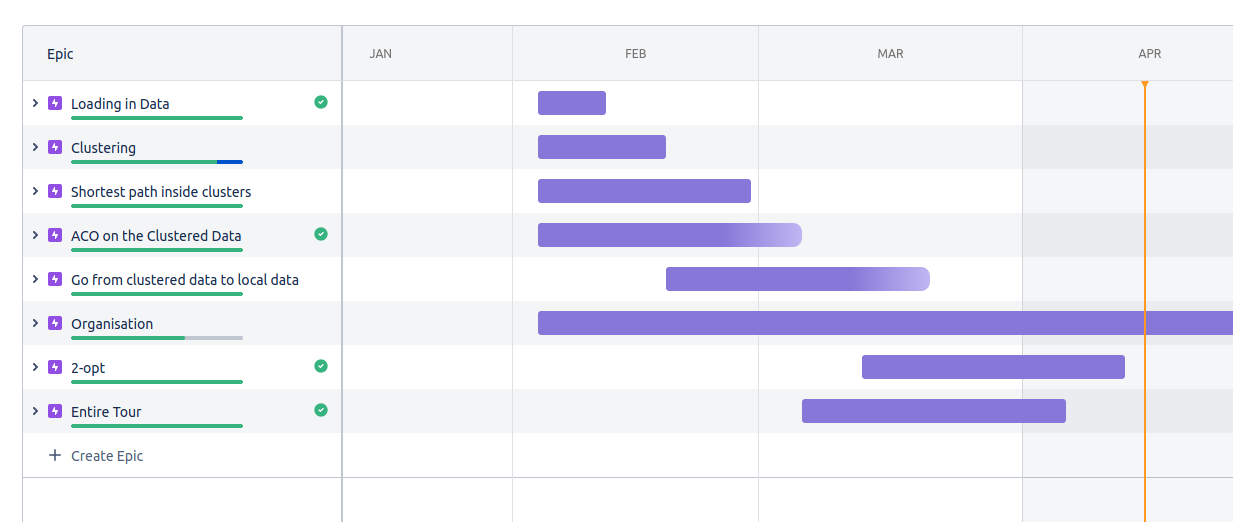
\includegraphics[width=\textwidth]{figures/jira_epics.png}
    \caption{Figure showing how the work was divided into epics in Jira, each epic had a number of tasks associated to it, when all of these tasks where completed the epic could be then be marked as done. This image was taken late into the project when most of the work had been done.}
    \label{fig:jira_epics}
\end{figure}

In Jira I assigned each task a story point estimate, this was a number between 0 and 3 that represented how much work that task would be to accomplish, 0 being very little work and 3 being a substantial amount of work normally several days. In Jira I could then generate a burndown report which could visualise how many story points I process through in a sprint and whether I was assigning myself a good amount of work each sprint. figure \ref{fig:jira_burndown} shows how this burndown chart looks in Jira.

\begin{figure}
    \centering
    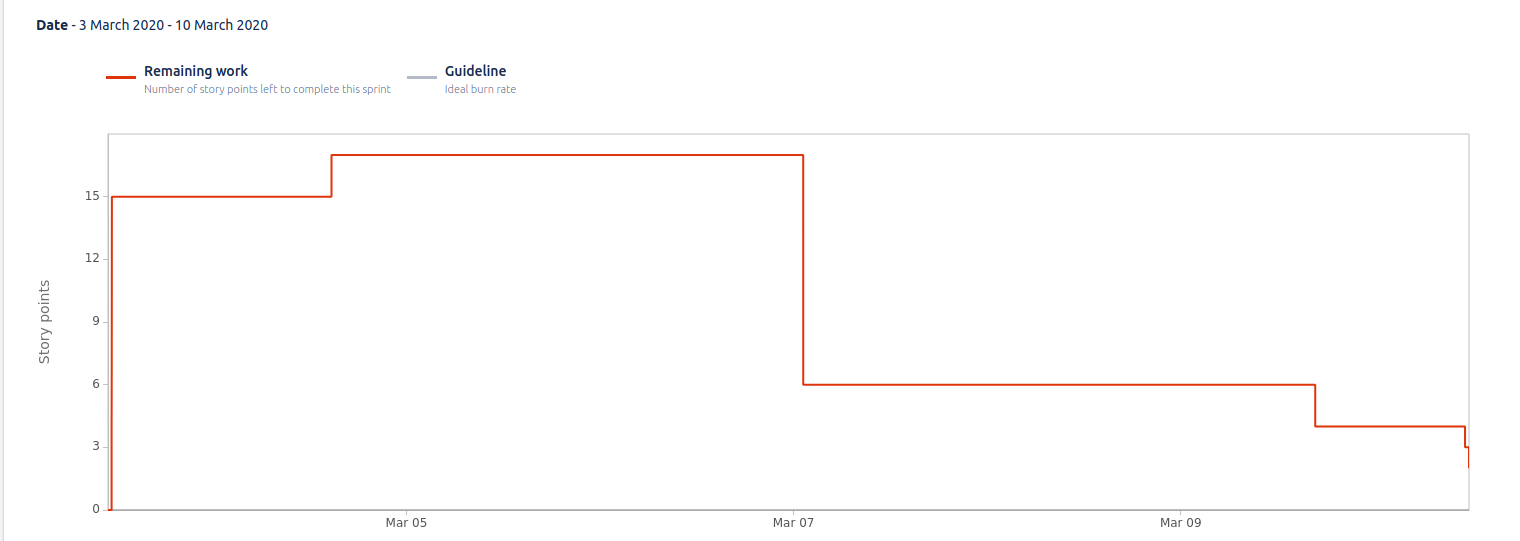
\includegraphics[width=\textwidth]{figures/jira_sprint_burndown.png}
    \caption{Figure showing Sprint burndown chart in Jira, this allows you to visualise how much work you normally accomplish on a given sprint and allow you to better plan your future sprints by allocating an appropriate amount of work. You can see in this sprint I started with 15 story points but after re-estimating a task that was raised to 17, I then managed to do most of that work and ended the sprint with 1 task left that had a story point estimate of 2.}
    \label{fig:jira_burndown}
\end{figure}

\begin{figure}
    \centering
    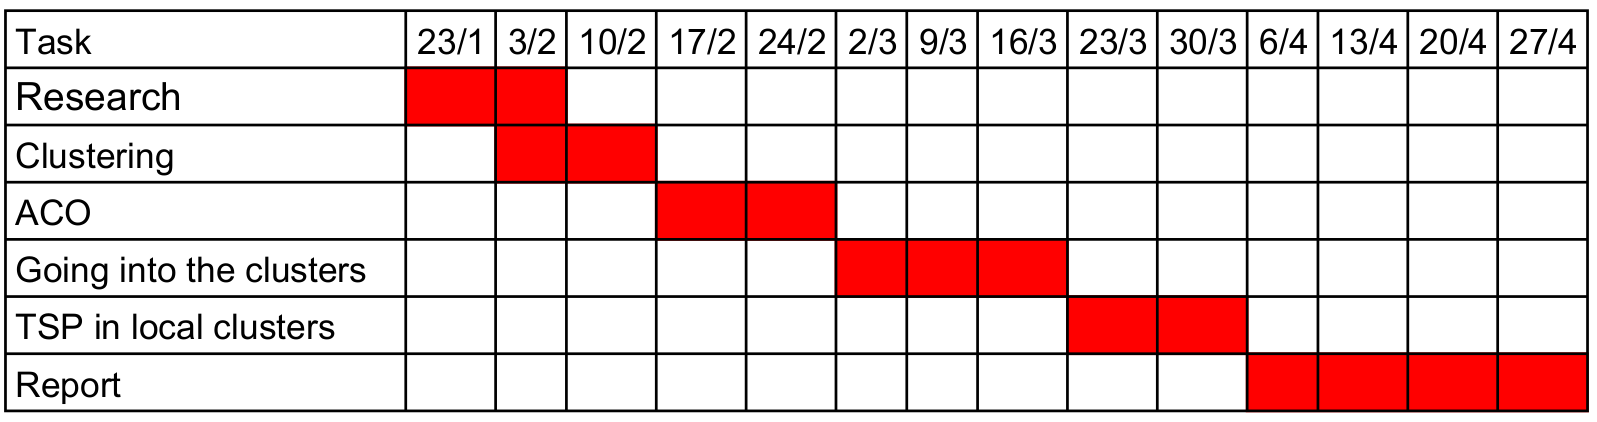
\includegraphics[width=\textwidth]{figures/initial_weekly_plan.png}
    \caption{Figure showing my initial weekly plan for the project, this was just a guiding view of the project and was meant as a way for me to monitor my progress, because I was using an Agile approach I didn't update this to include the deadline extension.}
    \label{fig:initial_weekly_plan}
\end{figure}
\chapter{Software Design, Implementation and Testing}

\section{Design}

\subsection{Tool Selection }

\subsubsection{Programming Language}

This project is focused on algorithm design and the performance of this algorithm, therefore I wanted a language that was rich in features but capable of high performance. The language needed to support object orientation and the necessary data structures that will aid in its implementation. Python, C++ and Java were all languages that I considered. I also wanted a language that had access to a huge number of libraries so that I could leverage these resources to more quickly and efficiently create my project, Python fulfills this requirement more than the other two. I also wouldn't need to create a web or GUI interface both of these are areas that Java is especially good at with the JavaFX library providing an easy way to implement graphical elements and the Spring package providing an easy way to create API calls for a web interface. Python and Java are slower than C++\cite{java_vs_c++}\cite{c++_vs_python} with Python being significantly slower. C++ is the better choice in terms of efficiency however I'm not aiming to create the fastest TSP solver only compare results so the speed benefit may not be required. C++ is also a less forgiving language where it's easier to make mistakes, if I wanted to use C++ then I would have had to spend a long time learning C++ in finer detail. 

I also wanted to be able to prototype solutions and due to Python's console support it is the language that would allow me to do this in the quickest and most efficient manner. With this in mind and its huge amount of library support especially in the area of data science/AI Python ended up being the better choice for me. 

\subsubsection{Development Environment}

I used the IntelliJ IDE PyCharm for this project\cite{pycharmide}, this IDE is easy to use but provides complex features that proved very useful, these features include; refactoring tools, thread concurrency monitoring, automated unit testing tools and automated virtualenv creation. I developed my project on Linux because I find that the features provided by the OS are conducive to productivity.

\subsubsection{Version Control System}
I used GitHub\cite{github} to host the code for my project and act as a Version Control System (VCS). This allowed for me to keep a backup of all the work I had done so if I needed to refer back to a change I'd made previously it was there and easy to access. GitHub is also really easy to setup and access and it can be connected to other applications for services like Continuous Integration.

\subsection{Overall Architecture}

My research required a piece of software be designed and built that could:

\begin{itemize}
    \item Load in TSP files
    \item Run the selected clustering algorithms over this data
    \item Run ACO over this clustered data
    \item Create a way to travel from one cluster to another in the tour
    \item Run a tour finding algorithm on the nodes inside each cluster
    \item Calculate the length of the tour
    \item Plot graphs relating to the tour
    \item Be able to execute the program as a script with CLI arguments
\end{itemize}

Based on this I created a list of requirements, (see Appendix \ref{appendix_requirements}). These were created at the start of the program and because I was using an Agile approach weren't kept fully up to date. but represent my thoughts about the software when I started building it which was a couple of weeks into the project.

My program works by:
\begin{enumerate}
    \item Loading in the data, this is stored as a TSPLIB95 file.
    \item Then clustering this and storing the clustered data.
    \item Run an ACO algorithm over the clusters to form a tour.
    \item Turning the ACO tour into a local tour by finding the entry and exit nodes for each cluster. These are the nodes that are closest to the next cluster in the tour.
    \item Find a tour through each of the clusters the tour starts at the entry node and ends at the exit node. This tour then gets recorded.
    \item Build a global tour by following through the ACO tour and substituting the clusters for the tours that were found in each cluster
    \item Run 2-opt over that tour
    \item Plot all the graphs
\end{enumerate}

Figure \ref{fig:run_diagram} illustrates how the program works, starting in section A the data is clustered, then in B the ACO tour is run, in C the entry and exit nodes are found for each cluster, and in section D tours are found for each cluster and 2-opt is run.

The output of the program gets saved to a log file for future reference.

\begin{figure}
    \centering
    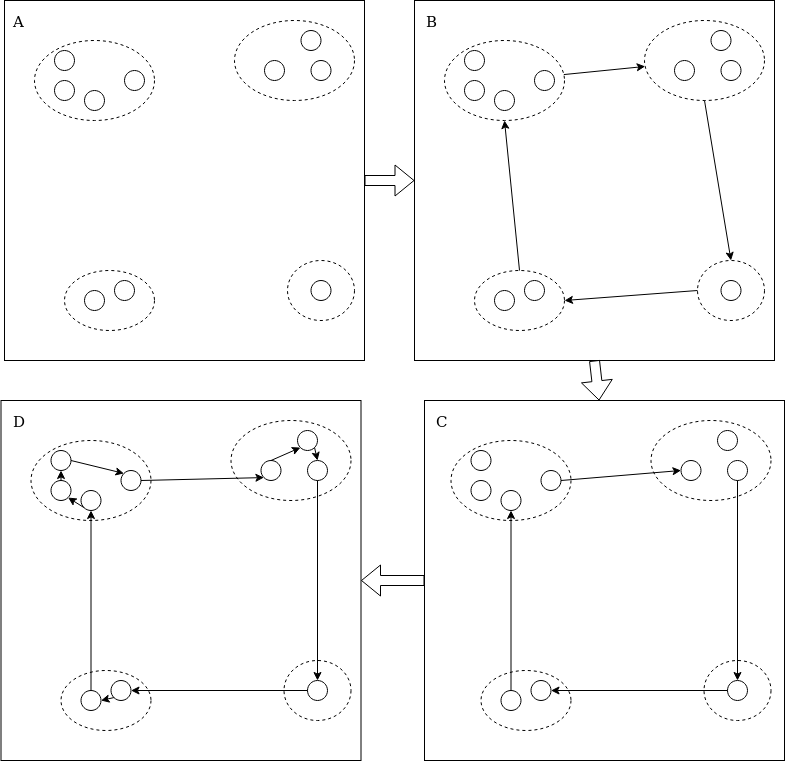
\includegraphics[width=\textwidth]{figures/diagram_design_how.png}
    \caption{This figure shows the steps the program takes: clustering, ACO tour, finding the entry and exit nodes for each cluster, and then finally finding tours within each cluster and bringing it together.}
    \label{fig:run_diagram}
\end{figure}

\subsubsection{Automated DBSCAN eps}

One of the areas that I was keen to improve on was the clustering, whilst I couldn't create a brand new clustering algorithm I did manage to automate a way to improve upon DBSCAN. As I mentioned previously DBSCAN requires a parameter called eps this is what allows for clusters to be found and is the most important factor to adjust when using the Algorithm. 

In \cite{optimal_eps_value_DBSCAN} Rahmah and Sitanggang figure out a way to find this value using a Nearest Neighbours approach. Their approach consisted of finding the distance between one node and all other nodes and then plotting these distances as a graph. This graph can be seen in figure \ref{fig:whole_eps_graph}, the optimal eps value is when the graph starts to curve. 

\begin{figure}[h]
    \centering
    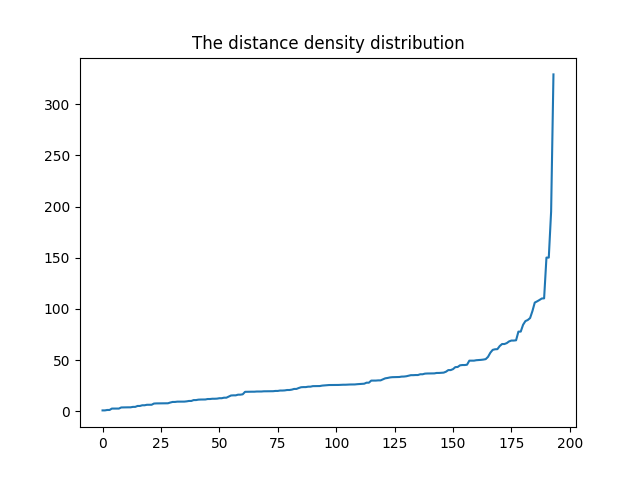
\includegraphics[width=\textwidth]{figures/eps_finder_graph_whole.png}
    \caption{Figure showing the graph that gets plotted when you find the distance from one node to every other.}
    \label{fig:whole_eps_graph}
\end{figure}

\begin{figure}[h]
    \centering
    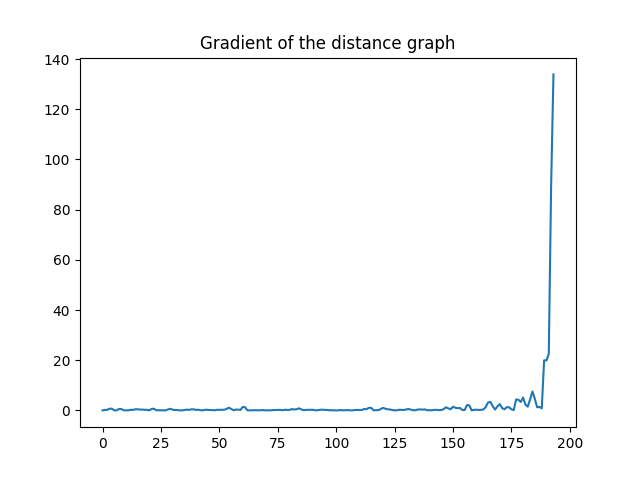
\includegraphics[width=\textwidth]{figures/eps_finder_graph_gradient.png}
    \caption{Figure showing the graph that gets plotted when you find the gradient of the nearest neighbour distances, this is the gradient of the graph shown in figure \ref{fig:whole_eps_graph}.}
    \label{fig:gradient_eps_graph}
\end{figure}

\begin{figure}[h]
    \centering
    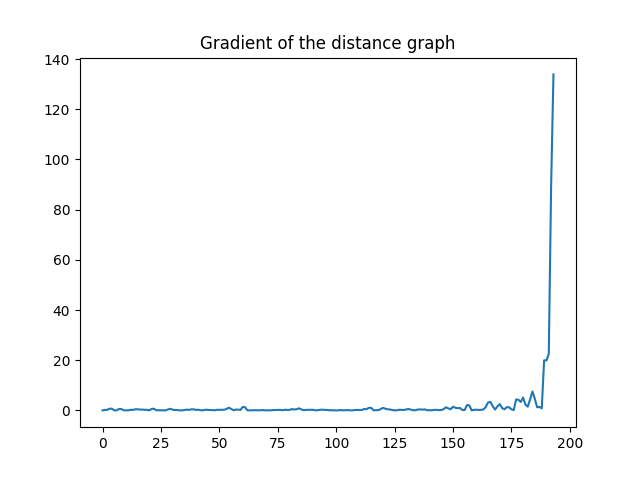
\includegraphics[width=\textwidth]{figures/eps_finder_graph_gradient.png}
    \caption{Figure showing the graph that gets plotted when you remove the last 1/7th of the data from the graph shown in figure \ref{fig:whole_eps_graph}.}
    \label{fig:cut_eps_graph}
\end{figure}

This can be found using the Nearest Neighbours algorithm present in Scikit Learn\cite{scikit_learn_nearest_neighbours}. To find the turning point of the graph I tried to take take the derivative and find where the change was biggest figure the graph of this is shown in figure \ref{fig:gradient_eps_graph}. This approach didn't work because if I were to take the largest gradient then I would end up with the eps value being the largest distance between two nodes which would result in DBSCAN finding a cluster that contained every node. To circumvent this I cut the last 1/7th off the graph and then found the highest point this graph is shown in figure \ref{fig:cut_eps_graph}. This approach worked for every piece of data that I tested it on however there may be data where this wouldn't work such as where the data increases in a circle out from central point.

\subsubsection{Script Interface}

I needed to create an easy way to run my program that would allow me to setup all my experiments and run them through quickly, I thought about using a web interface or building a GUI for this that would allow runs to be queued up and executed when the previous one had finished but I decided against this because I thought that it would over-complicate things and I wanted to focus on the research side. Instead I made it execute like a script. A script allows for queuing tasks to be run later and would be easier to implement giving me more time to focus on the experiments to be run.

The program is constructed to allow for command line arguments to be given, these are available in Table \ref{tab:commandargs} in Appendix \ref{apd:commandline_arguments}. The arguments allow for every aspect of the program to be controlled such as: the arguments provided to the clustering algorithms and the ACO algorithms, the input file to read, output folder, the clustering and ACO algorithms to use, and it allows for various features to be turned on or off. 

Not all of these parameters have to be given every time you run the program only a few are essential and the parameters that are optional and aren't set are auto-populated from a list of default values, these default values are also shown in the table.

To hold these options values I had an Options class, this made use of pythons ability to have function arguments hold default values, when this class was constructed all the command line arguments were passed to it and the ones that weren't provided were taken from the default values file.

\section{Implementation}

There are several key sections to my project. This section discusses the implementation of them, I made use of existing libraries in my project to speed up the work and allow me to focus more on the research. Some of these libraries needed changes so they worked the way I wanted them to and so they had all the features I needed. 

\subsection{Loading TSP Files}

As I mentioned previously I'm using common TSPLIB files these files can hold a lot of data and creating a parser that can deal with all of that would be a tremendous amount of work. I found the library tsplib95\cite{tsplib95} this can read in all sorts of TSPLIB files and works very well. This library contains lots of helpful utility functions that I thought may be useful, features such as: turning the problem into a networkx\cite{networkx} graph and creating distance matrices for the data.

When the file gets loaded in I turn it into a numpy\cite{numpy} array, it has to be a numpy array in order to work with the clustering algorithms. 

\subsubsection{Generating TSP Data}

Lots of the TSP data available contains many thousands of nodes and because of their size they take a long time to run. I wanted to test my algorithm on smaller problems that contained a few hundred nodes. In order to do this I had to create my own TSP data this was a straightforward task, I created a Python file that had several parameters: number of nodes, number of cluster, size of clusters and the scale that the nodes should be plotted on. This then randomly places nodes around the graph, to create clusters it randomly picks some nodes to act as cluster centres and places nodes around them.

The TSPs that are generated are modelled after 'world' TSPs in that they mimic real world clusters. They are not meant to look like VLSI data.

\subsection{Clustering}

The clustering algorithms that I wanted to implement were all available as part of the Scikit Learn library. In order to use this the data had to be available as a numpy array so I had to ensure that when I read the data I transformed in into that type of array. 

Once the data is clustered I needed a way to hold all the data, for this I made two classes: one called ClusteredData and the other called Cluster. ClusteredData holds all the nodes in the problem and all the clusters that have been created, there are two sorts of clusters that it can hold: full clusters and unclassified node clusters. Some of the clustering algorithms return nodes that don't fit into any specific cluster so I call these unclassified node clusters, these are treated differently because they don't need a tour created for them or entry/exit nodes calculated. 

\subsection{Graph Plotting}

I used the library Matplotlib\cite{matplotlib} to do all my graph plotting, it's very feature rich and allowed me to easily create graphs, so made sense for me to use it instead of creating my own plotting library. The graphs are plotted at the end of the run so as not to slow down the program and interfere with the run time statistic.

The following graphs are plotted:

\begin{itemize}
    \item ACO tour of the clustered data
    \item All the nodes in the problem
    \item The data after it had been clustered
    \item The tour for each cluster
    \item The final tour before 2-opt
    \item The final tour after 2-opt
\end{itemize}

\subsubsection{Visualiser of 2-opt and ACO Tour Improvements}

In addition to the graphs that get plotted two videos are also created one that shows the incremental improvement that 2-opt makes and another that shows the incremental improvement of ACO. This works by having a class called TourImprovementAnimator that both 2-opt and ACO have a reference to, every time there is an improved tour they record this on the object.

At the end of the program when the solution has been found the graphs get plotted. The TourImprovementAnimator plots all the tours and saves them to a folder using Matplotlib\cite{matplotlib}. This plotting makes use of the Python multiprocessing library which greatly speeds this process up, these images are then read back in and placed into a video using the library imageio\cite{imageio}.

\subsection{ACO}

I have used two ACO libraries; ACOPY\cite{acopy} and an ACO algorithm that makes use of multi-threading\cite{multithreaded_aco}. ACOPY was available as a dependency that I could install via pip, the other was not and so I had to pull the code from its GitHub repository and use it that way. The code was written for Python 2 and since I was using Python 3 I had to make some small changes to it in order to get it to work, these were mostly upgrading the tests and changing some parameters to be lists. 

ACOPY allowed you to add plugins to extend the functionality of the algorithm. The plugins are called at various points and allow for changes to be made to various parts of the algorithm. I created two plugins the first one records data about the current iteration including the tour and the length of this tour, the second one records the tour after every iteration into a TourImprovementAnimator object.

The other library doesn't have plugin functionality or anything similar so I had to modify the code to get it to print out the data after every iteration and record the tour into a TourImprovementAnimator.

I implemented the second library because when I was running ACOPY I noticed that it took a while to run and only used one core so I found the multi-threaded ACO algorithm to see if it helped speed the program up

\subsection{2-opt}

2-opt is a simple local search algorithm, it can be seen as a way to smooth out a tour by deleting crossed over paths, this can be seen in figure \ref{fig:2-opt-example}. 2-opt works by removing two edges from the tour and reconnecting them, it only does this if the resultant tour will be shorter. The pseudo code is shown in Figure \ref{fig:2-opt-epseudo-code}. A complete 2-opt search will swap and compare every pair of nodes, this technique can be applied to any graph routing problem. 2-opt is applied to improve existing routes therefore it is bound by the structure that it is given, because of this it is only only able to find the locally optimal solution not the globally optimal solution for the problem. 

\begin{figure}
    \centering
    
\includegraphics[width=\textwidth]{figures/2-opt-example.png}
    \caption{An example of 2-opt running over a tour. It has swapped the connection b-e and f-c which has removed the cross and made the tour shorter.\cite{2_opt_example_picture}}
    \label{fig:2-opt-example}
\end{figure}

\begin{figure}
\begin{verbatim}
repeat until no improvement is made {
    start_again:
    best_distance = calculateTotalDistance(existing_route)
    for (i = 1; i <= number of nodes eligible to be swapped - 1; i++) {
        for (k = i + 1; k <= number of nodes eligible to be swapped; k++) {
            new_route = 2optSwap(existing_route, i, k)
            new_distance = calculateTotalDistance(new_route)
            if (new_distance < best_distance) {
                existing_route = new_route
                best_distance = new_distance
                goto start_again
            }
        }
    }
}

procedure 2optSwap(route, i, k) {
    1. take route[0] to route[i-1] and add them in order to new_route
    2. take route[i] to route[k] and add them in reverse order to new_route
    3. take route[k+1] to end and add them in order to new_route
    return new_route;
}

\end{verbatim}
\centering
\caption{The pseudo code for the 2-opt local search algorithm.\cite{2_opt_pseudo_code}}
\label{fig:2-opt-epseudo-code}
\end{figure}

My implementation is modified slightly because TourImprovementAnimator records the tour each time an improvement is found.

The run time of 2-opt is quite high, it could be improved through the use of multi-threading so that the load was spread over the entire processor. However I was unable to do this in the time I had and couldn't find any references to it online when I looked.

\subsection{Tours Within Clusters}

When the ACO tour over the clustered data has finished I needed a way of turning the ACO tour into a tour that covered every node. The first thing that happens here is the nodes to move from one cluster to the next are found. These are called the entry and exit nodes and are found by finding the two closest nodes between each cluster. 

Tours are then found in every cluster going from the entry node to the exit node, these tours can be found by using ACO and by using a greedy nearest neighbour heuristic. The ACO approach uses the ACO algorithm that the user has specified, when this is used the end node is not included in the ACO search this is because the ACO algorithm has no way to specify the end node. To get around this I add the end node on when the search has finished however this can cause bad unoptimised tours.

The heuristic approach works by starting at the clusters entry node and travelling to the nearest node that it hasn't previously visited and travelling to the exit node last.

One problem I encountered when implementing this was that when all the tours were being combined some tours might end up reversed and this would cause what should be the exit of the cluster becoming the start node. This really affected the length of the tour. To mitigate this I implemented a dictionary that mapped the cluster to the node that it connected to. Then when the global tour gets constructed it checks this dictionary to ensure that everything is in the right order and if it isn't then it reverses the tour so it is. This solved my issue but isn't a great solution and I should have spent more time investigating this and putting in place a more robust solution but this does solve the problem.  

\section{Testing}


\subsection{Overall Approach to Testing}

I wanted as much automated testing as possible because I find it is incredibly useful to be able to test software every time a change is made. This really allows one to be confident in the changes one is making. Due to the complicated nature of my project and the amount of time that is required for a run to successfully take place I knew that not everything would be able to be testing in this fashion.

I utilised quite a lot of informal testing, every time a new change was made I ran the code through and ensured that everything was working as it should.

\subsection{Automated Testing}

I used the continuous integration platform Travis-CI\cite{travis_ci} to automatically run my tests. Travis links to your GitHub profile and when you a new commit is pushed it starts a build process. It reads a configuration file located in the root of the repository called .travis.yml which contains all the build instructions. My file told Travis that Python was being used, to install the requirements listed in requirement.txt and run the tests using pytest. If the tests passed then the build was successful otherwise the build failed and I was notified. 

The automated tests I wrote focused on loading in data and the ClusteredData class, lots of tests were also provided from the multithreaded ACO algorithm which I included.


\chapter{Results and Conclusions}

When the algorithms were tested each one was run ten times. This was to ensure that the results that I was getting were accurate. I did not want to only capture one data point because if I had done so then I might have captured a very good ACO run that gave a short route, this would have not been representative of the overall algorithm. The full result tables are provided in Appendix \ref{apd:result_tables}.

The TSP problems called 100\_node 200\_node and 300\_node were created by me using my TSP file generator. They were modelled after world TSP data. The remaining three TSP files mentioned are VLSI TSP data.

I did make every effort to ensure that my computer was idle when running these tests but some results do stick out as outliers because of either they're much higher or much lower run times. I would like to rerun these tests but due to the high run times of these algorithms I will not be able to do this. 

For the PBM436 TSP I have only managed to run it through once for the ACO only part. I ran out of time to run it the remaining nine times, it took 84474 seconds to run through which is nearly 24 hours. I would have liked to run this through multiple times so that I could be sure that this is an accurate piece of data but in this case it was not possible.

\section{Does clustering allow ACO to be applied to larger problems?}

This question was about seeing if clustering sped up ACO enough for ACO to be applied to larger problems. To see if this was the case I ran six pieces of TSP data: 100\_node, 200\_node, 300\_node, XQF131, XQG237 and PHM436. These are half VLSI data and half self created world data. For each piece of data I ran it using a sole ACO approach and measured the time it took to run, I also ran it using four clustering algorithms: DBSCAN, OPTICS, Affinity Propagation and K-Means. For DBSCAN I used my approach that estimated the eps value and for K-Means I set the node count to 20. Each test was ran ten times and these results are the average of those runs.

It ran with the following ACO parameters: 300 iterations, number of ants is number of nodes divided by 1.5, $\alpha$ is 1, $\beta$ is 10, $\rho$ is 0.4 and $Q$ is 1000.

\begin{longtable}[c]{|p{2cm}|p{1cm}|p{2cm}|p{2cm}|p{3cm}|p{2cm}|}
\hline
\multicolumn{6}{|c|}{The Ratio of Running Speed}                                     \\ \hline
\endhead
%
\multicolumn{6}{|c|}{Ratio = Time(ACO)/Time(Algorithm)}                              \\ \hline
          & ACO   & ACO-DBSCAN & ACO-OPTICS & ACO-AFFINITY-PROPAGATION & ACO-K-MEANS \\ \hline
100\_node & 1.000 & 8.857      & 8.377      & 6.454                    & 11.159      \\ \hline
200\_node & 1.000 & 16.500     & 18.540     & 18.266                   & 32.041      \\ \hline
300\_node & 1.000 & 13.199     & 8.415      & 28.652                   & 39.697      \\ \hline
xqf131    & 1.000 & 7.110      & 3.814      & 13.679                   & 20.944      \\ \hline
xqg237    & 1.000 & 8.437      & 3.317      & 29.225                   & 41.343      \\ \hline
pbm436    & 1.000 & 9.396      & 5.022      & 53.098                   & 58.494      \\ \hline
\caption{This table shows the run time ratios that were achieved. The run time ratio is a measure of how much faster that algorithm is when compared to an ACO only approach, a value of 16.5 means that that particular algorithm is 16.5 times faster than ACO only. }
\label{tab:run_time_table_question_1}\\
\end{longtable}

Table \ref{tab:run_time_table_question_1} shows the run time results that were achieved when running these tests.

As the size of the problem increases so too does the improvement gained through the use of clustering, due to the run time of ACO scaling to the square of the number of nodes in the problem it's very important to reduce the number of nodes that ACO runs over in at any particular point. From a run time perspective the best performing algorithms immediately reduce the number of nodes. DBSCAN and OPTICS both have the concept of noise which has the effect of ACO initially running over more nodes. For the 300 node problem DBSCAN generated 21 clusters and 75 nodes and OPTICS generated 20 clusters and 103 nodes, therefore for these two algorithms the run times are a lot higher. Looking at the 300\_node problem even though DBSCAN and OPTICS both have have more nodes for ACO to initially run over they still give significant performance gains.

As the number of nodes increase K\_Means really shows how much it can improve. In the 300\_node problem it generates 20 clusters of roughly equal size, the largest cluster it generates contains 31 nodes. This causes a massive decrease in run time because ACO is running over fewer nodes at any one time.

My results shows that by combining ACO with clustering a considerable run time improvement can be made against a pure ACO approach. This is consistent with what was found in \cite{pang_chao-yang_ben-qiong_zhang_jie_wei_shan_zheng-chao_2014}, here they also showed that ACO can be beaten by clustering algorithms although the clustering algorithms they chose are faster and beat ACO by a higher factor. The only clustering algorithms that we both use is K-Means and our results are very similar for a number of TSPs. They do differ slightly but this can be because of any number of reasons, they don't provide a k value so they may be splitting into more clusters which will slow the process down. They also don't say what type of data these are, there is a link to the data but as of 7th May that link doesn't appear to be working so I can't see how complex or what type of TSP problem they are running.

The clustering algorithms seem to have very different results when running on VLSI problems, OPTICS and DBSCAN both perform very poorly in this situation when compared to 'world' TSP data. It seems like these clustering algorithms are poorly suited to clustering this type of data, the structure of VLSI data performs poorly when clustered with these conventional clustering algorithms. DBSCAN and OPTICS don't manage to place many nodes into clusters they regard most nodes as noise. This causes the run time of ACO to increase as it is now run over more nodes. DBSCAN performs better than OPTICS, the automated distance finding for OPTICS is not suited to the patterns presented in VLSI data. I can not make direct comparisons between my runs of VLSI data and the aforementioned paper because I do not know the types of the TSP data that they have used.

K-Means and Affinity Propagation have no problems dealing with VLSI data they are able to cluster it and give very good results.

\section{To what effect do different clustering algorithms have on the quality and run time of the solution?}\label{sec:question2}

This question was about seeing the effect that the clustering algorithm had on ACO, do particular clustering algorithms perform better when combined with ACO to solve a TSP and are they therefore better suited to solve this problem.

To see if there was a clustering algorithm that was better than any others I chose four algorithms: DBSCAN, OPTICS, Affinity Propagation and K-Means. I chose these algorithm because K-Means is similar to Affinity Propagation except that it requires a parameter k, the number of nodes, at the start. DBSCAN and OPTICS are also similar, they both have the concept of noise, except OPTICS is designed to be more automated. When I run DBSCAN I used my version which found an optimal eps value from the data. 

It ran with the following ACO parameters: 300 iterations, number of ants is number of nodes divided by 1.5, $\alpha$ is 1, $\beta$ is 10, $\rho$ is 0.4 and $Q$ is 1000. The K-Means k value was 20.

\begin{figure}
    \centering
    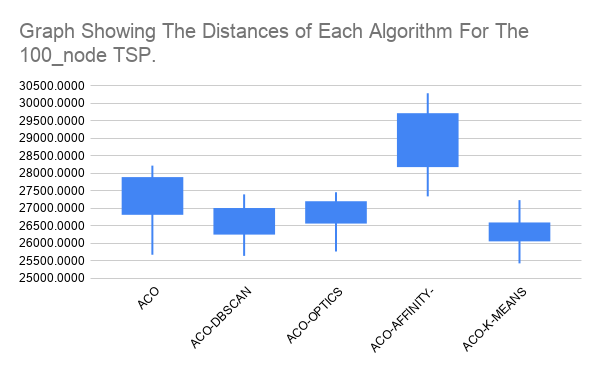
\includegraphics[width=\textwidth]{figures/distance_100_node_graph.png}
    \caption{Box plot showing the distances that were achieved when running the algorithms over the 100\_node TSP. The cut off label reads ACO-Affinity-Propagation.}
    \label{fig:distance_100_node}
\end{figure}

\begin{figure}
    \centering
    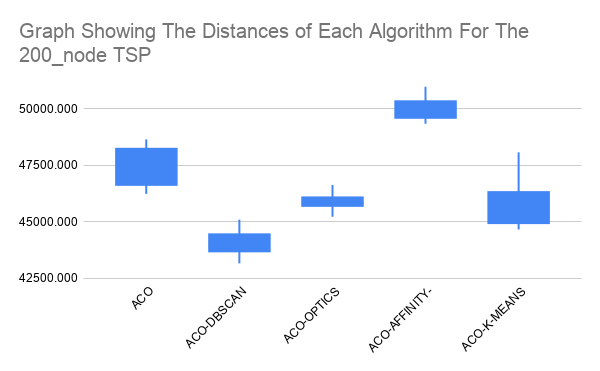
\includegraphics[width=\textwidth]{figures/distance_200_node_graph.png}
    \caption{Box plot showing the distances that were achieved when running the algorithms over the 200\_node TSP. The cut off label reads ACO-Affinity-Propagation.}
    \label{fig:distance_200_node}
\end{figure}

\begin{figure}
    \centering
    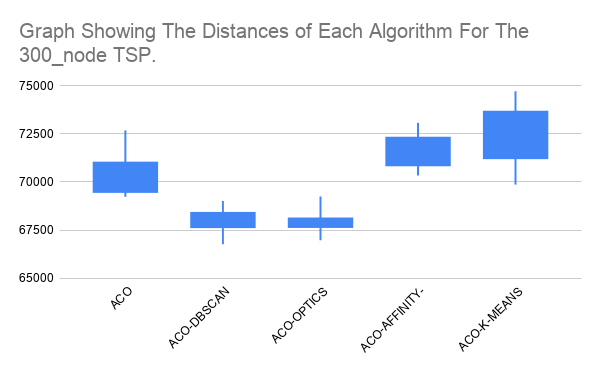
\includegraphics[width=\textwidth]{figures/distance_300_node_graph.png}
    \caption{Box plot showing the distances that were achieved when running the algorithms over the 300\_node TSP. The cut off label reads ACO-Affinity-Propagation.}
    \label{fig:distance_300_node}
\end{figure}

\begin{figure}
    \centering
    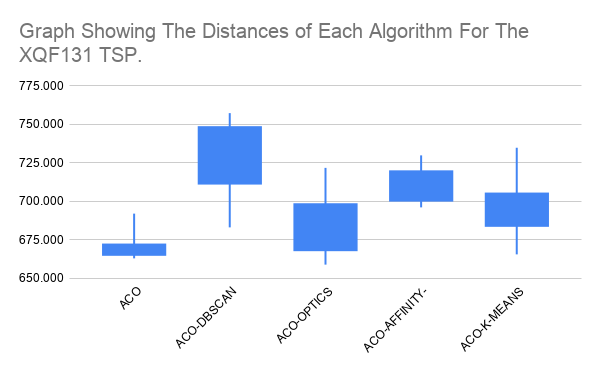
\includegraphics[width=\textwidth]{figures/distance_xqf131_graph.png}
    \caption{Box plot showing the distances that were achieved when running the algorithms over the XQF131 TSP. The cut off label reads ACO-Affinity-Propagation.}
    \label{fig:distance_xqf131}
\end{figure}

\begin{figure}
    \centering
    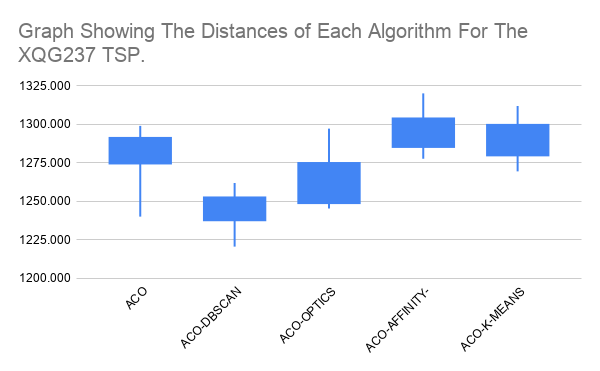
\includegraphics[width=\textwidth]{figures/distance_xqg237_graph.png}
    \caption{Box plot showing the distances that were achieved when running the algorithms over the XQF237 TSP. The cut off label reads ACO-Affinity-Propagation.}
    \label{fig:distance_xqg237}
\end{figure}

\begin{figure}
    \centering
    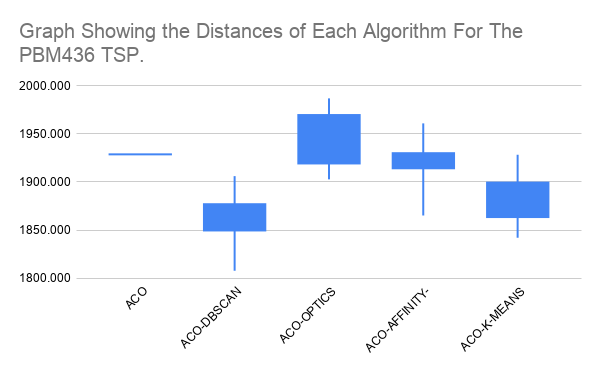
\includegraphics[width=\textwidth]{figures/distance_pbm436_graph.png}
    \caption{Box plot showing the distances that were achieved when running the algorithms over the PBM436 TSP. For this TSP ACO was only run once due to its incredibly long run time. The cut off label reads ACO-Affinity-Propagation.}
    \label{fig:distance_pbm436}
\end{figure}

Figures \ref{fig:distance_100_node}, \ref{fig:distance_200_node}, \ref{fig:distance_300_node}, \ref{fig:distance_xqf131}, \ref{fig:distance_xqg237} and \ref{fig:distance_pbm436} show the distances that were achieved for these algorithms. These graphs plot the minimum value achieved, the lower quartile, the upper quartile and the maximum value that have been achieved. These quartiles show the spread of the results, the smaller spread would show consistency amongst the results. 

Looking at the world TSP data Affinity Propagation consistently performs worse with poorer results, this could be because it splits the data up into fewer nodes so ACO has less data to work with. Fewer nodes means that it's simpler for ACO to compute the tour but this does mean you don't get the benefits that path finding with ACO provides. Affinity propagation may produce clusters that do not fit the structure of the data very well, it attempts to combine too many nodes into a single cluster which negatively affects the cluster  path finding.

DBSCAN and OPTICS both split the data up into many more nodes than any other algorithm because they support the concept of noise, this leads to ACO initially having more nodes to run over which generates better tours and possibly a better structure. This allows the clusters to expand in a way which means the tour is more optimal.

K-Means performs very well especially on the smaller problems, it does trail off when the number of nodes are increased though. This leads to me thinking that there is an optimal K value depending on the size of the problem, this would be an interesting question to explore. 

For VLSI data all the algorithms seem to be very equal this may be because these algorithm are not really suited to the shapes and complexities of this type of data. The most optimal routes for this types of data follow the paths that the nodes lay out, however the clustering algorithms expand circularly which influences the ACO tour to also follow that pattern. This is why the ACO only tour performs very well on the smaller problem, if it was run over more iterations then it would have also performed well for the larger problems. For TSP XQG237 ACO can perform very well but is unlikely to and this is down to the number of iterations it has run and general luck that the ants have picked good routes.

Optics performs very poorly on this VLSI data, it is unable to find clusters within the data and returns most of the nodes as unclusterable noise. This does mean that it provides tours of reasonable length because ACO is run over most of the nodes in the problems and isn't bound by any bad clustered structures that OPTICS has returned.

DBSCAN, mostly does the best job. It seems to do a good job finding reasonable clusters for this data, though there are still a lot of unclusterable nodes although fewer than OPTICS this does lead to better tours being found as well as lower run times. For XQG237 OPTICS finds 15 clusters and 129 unclusterable nodes, DBSCAN finds 30 clusters and 69 unclusterable nodes, the clusters that DBSCAN finds map more closely to the patterns in the data. There are a lot more clusters that closely follow the lines presented in the data. Figure \ref{fig:xqg237_optics} and \ref{fig:xqg237_dbscan} shows the clustering that was achieved with DBSCAN and OPTICS and you can see just how much better DBSCAN is, the clusters are smaller and follow the way the data flows. DBSCAN is a lot better at finding clusters with this challenging data.

\begin{figure}
    \centering
    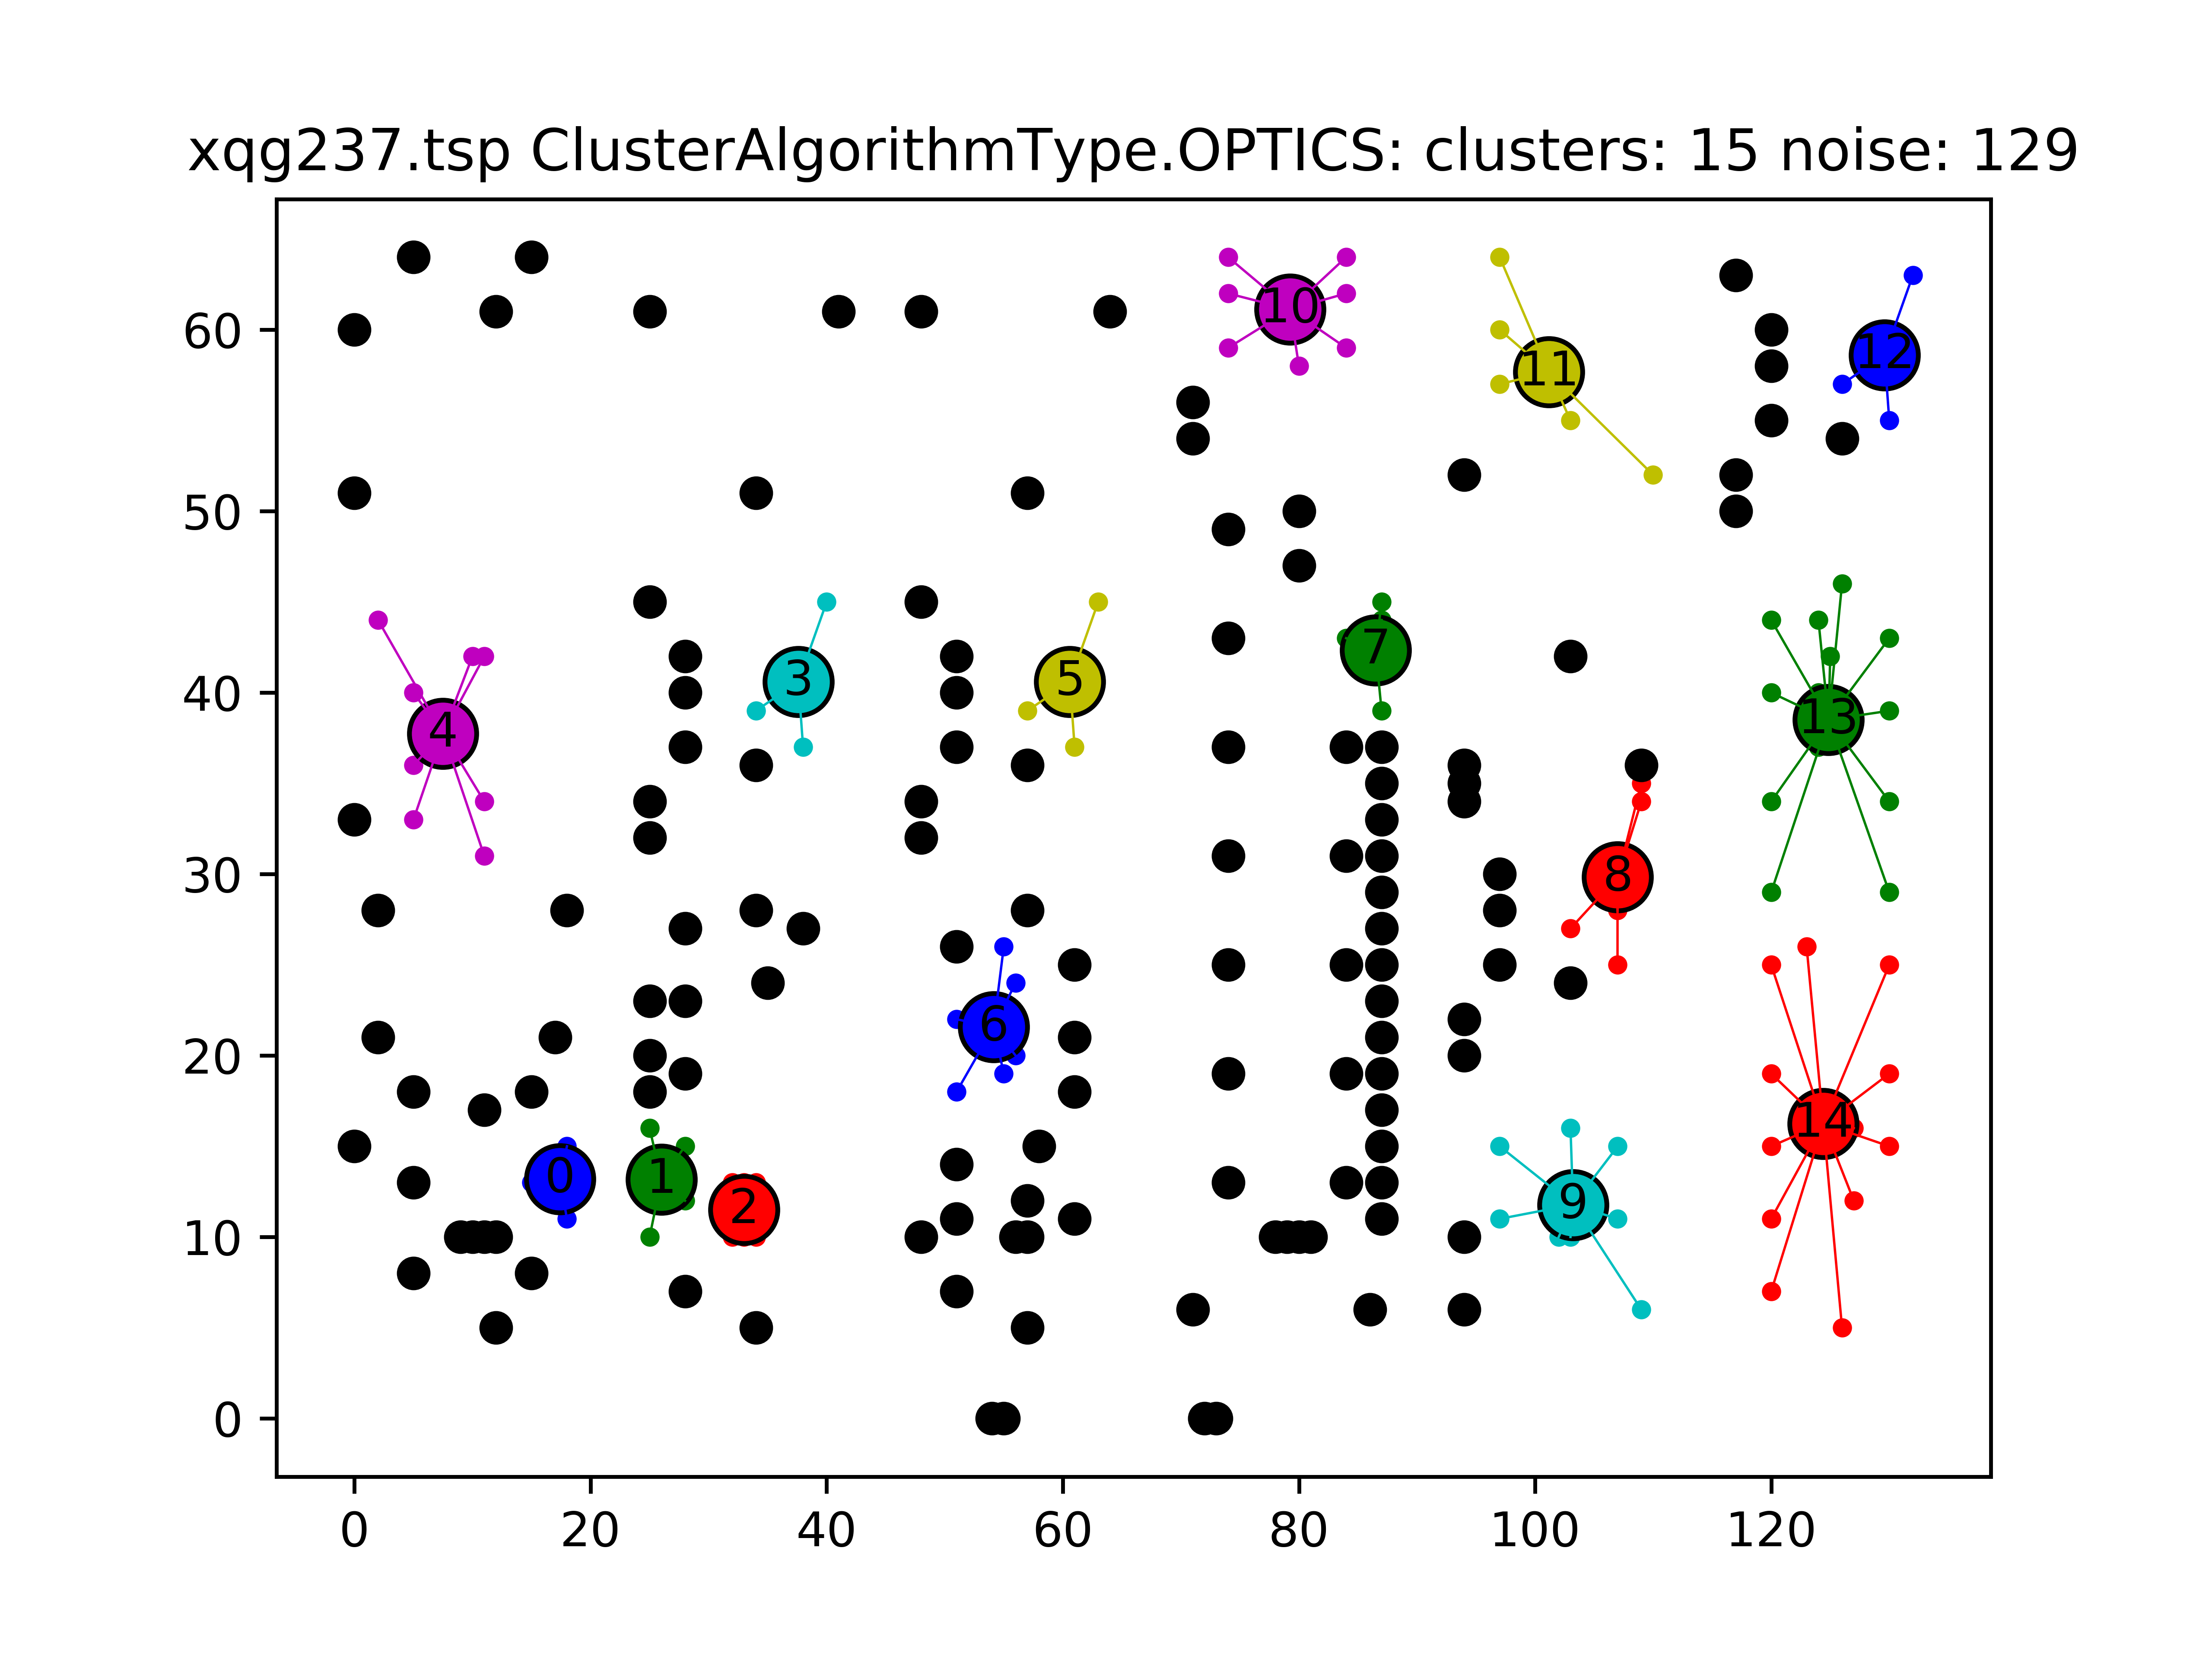
\includegraphics[width=\textwidth]{figures/xqg237_OPTICS.png}
    \caption{The OPTICS clustering for XQG237.}
    \label{fig:xqg237_optics}
\end{figure}

\begin{figure}
    \centering
    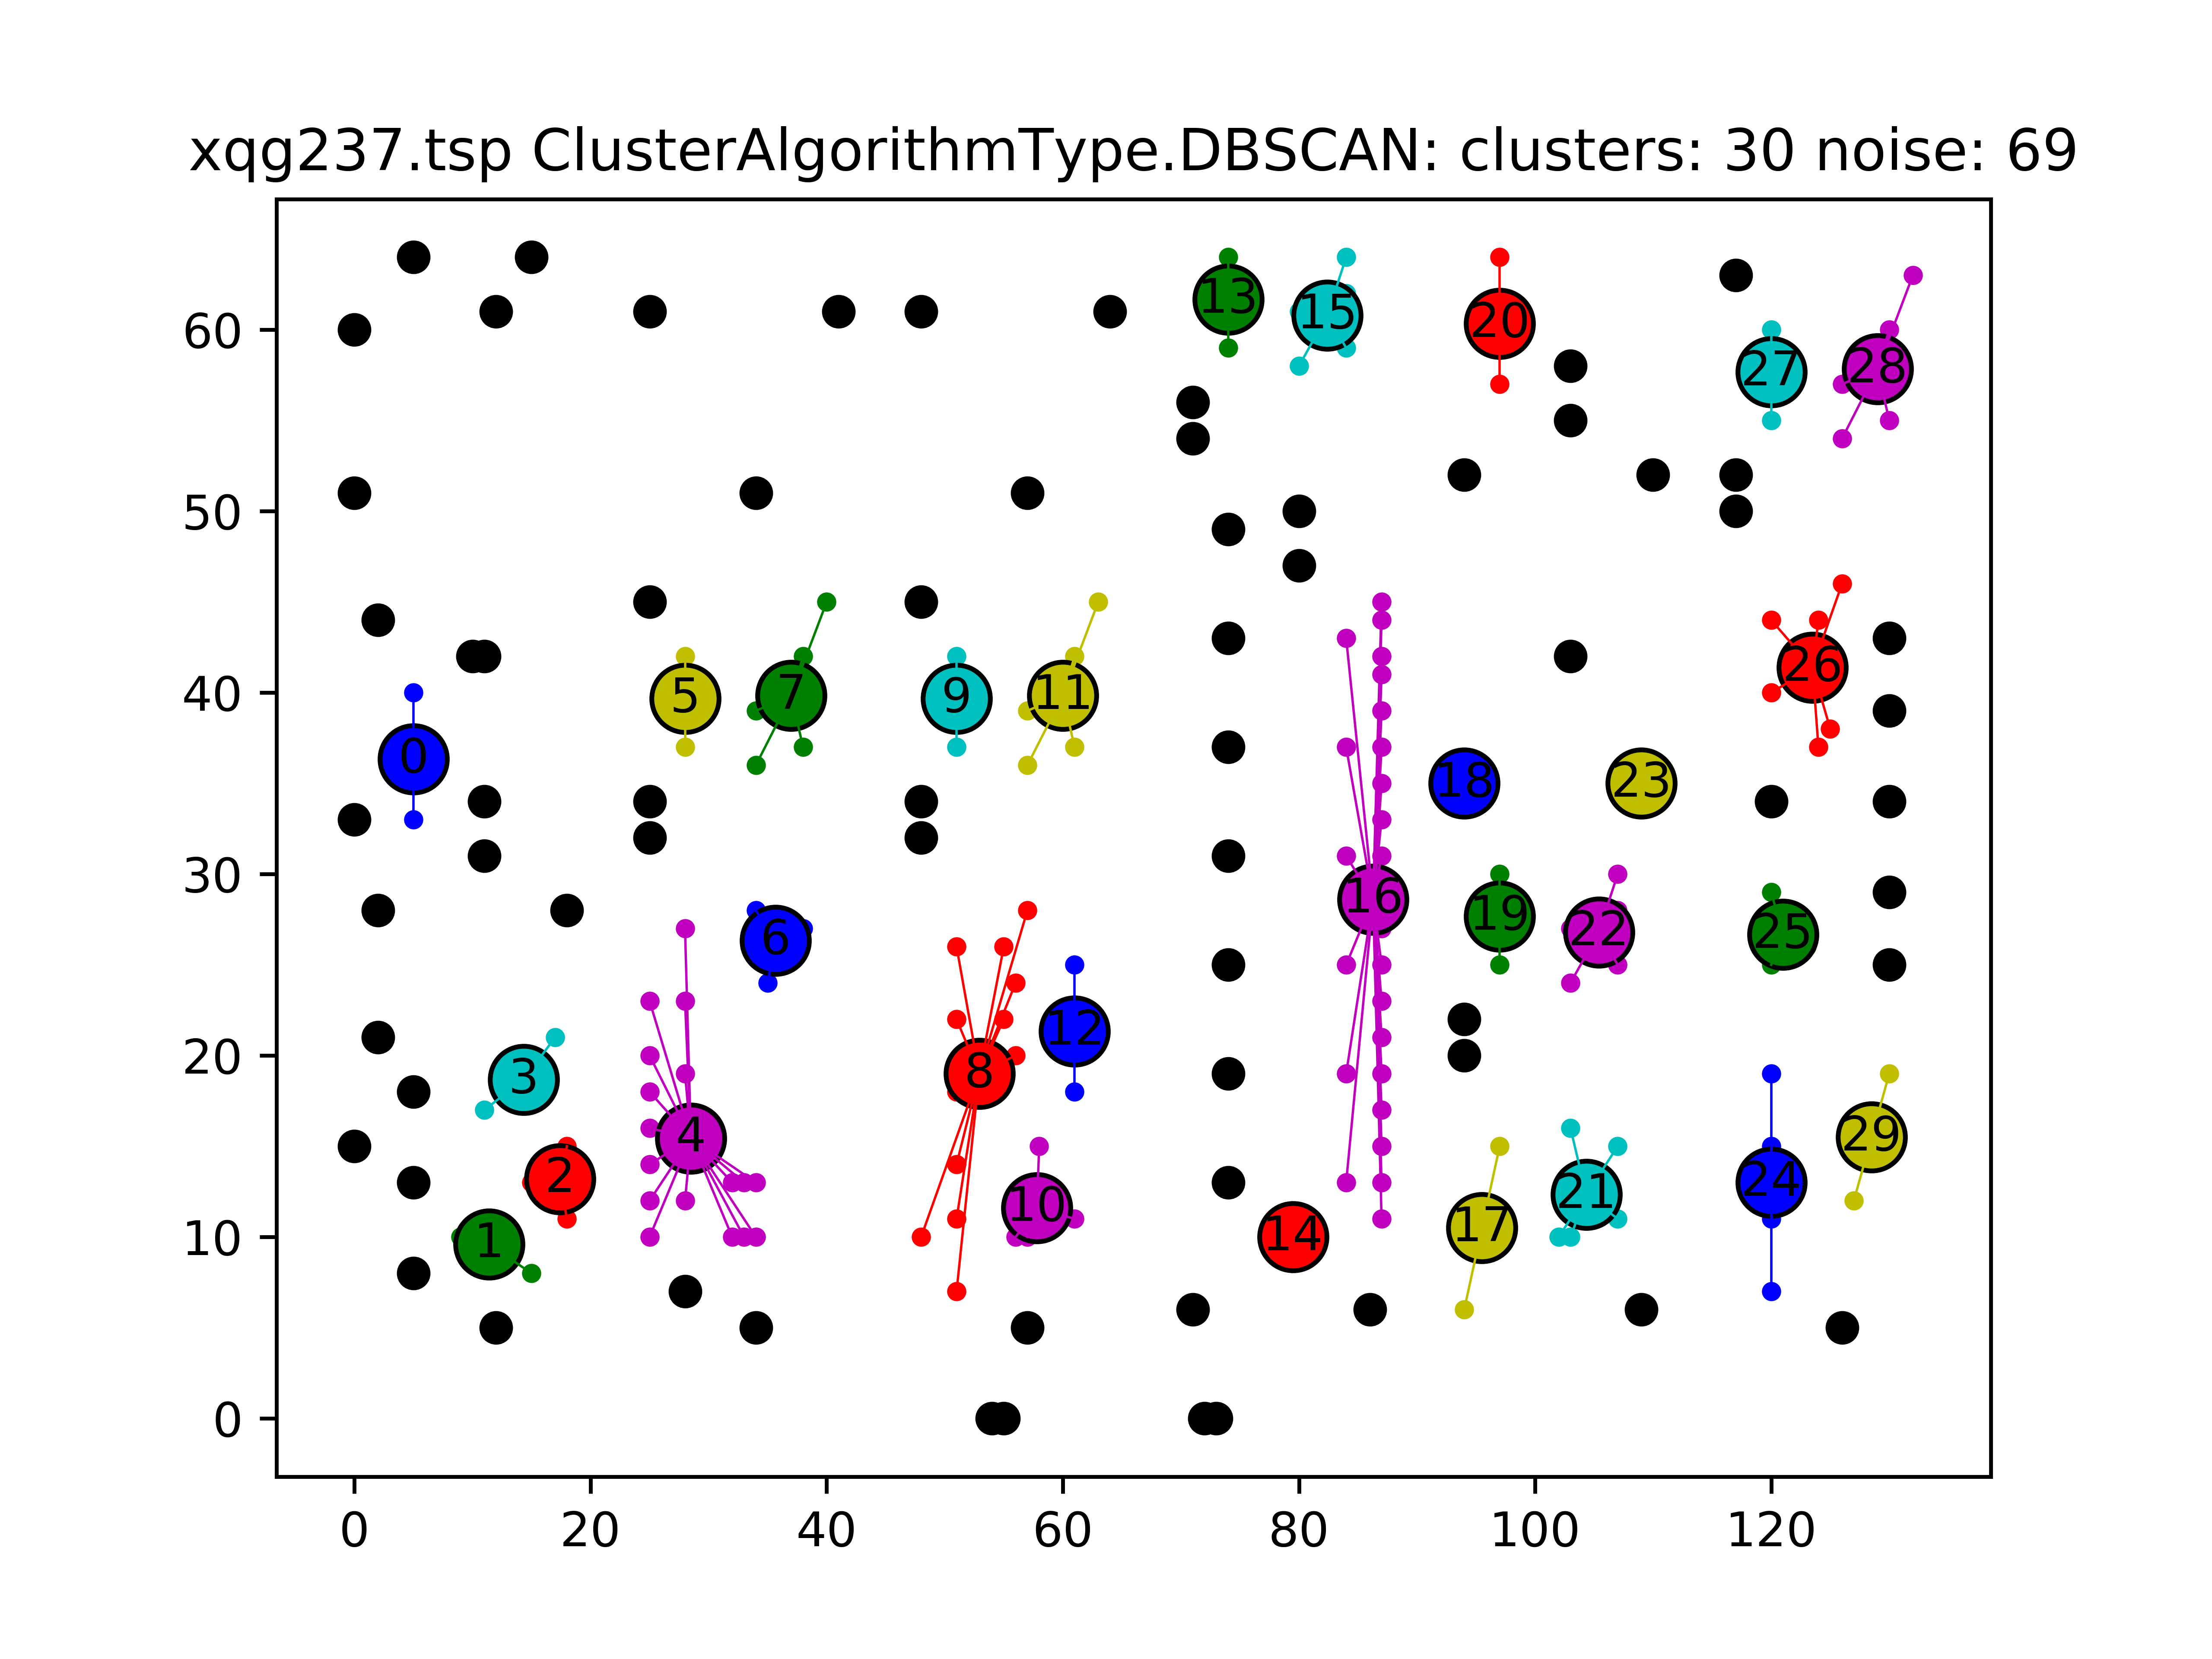
\includegraphics[width=\textwidth]{figures/xqg237_DBSCAN.png}
    \caption{The DBSCAN clustering for XQG237.}
    \label{fig:xqg237_dbscan}
\end{figure}

For VLSI data K-Means performs admirably with a very low run time, it benefits from the many small clusters which greatly reduce the run time of ACO. It doesn't pick out the best patterns in the data as it expands circularly but because a k value of 20 was used there are many clusters and they are all of relatively small sizes.

\begin{longtable}[c]{|p{2cm}|p{1cm}|p{2cm}|p{2cm}|p{3cm}|p{2cm}|}
\hline
\multicolumn{6}{|c|}{The Ratio of Distance To Running Speed}                          \\ \hline
\endhead
%
\multicolumn{6}{|c|}{Ratio = Distance of Algorithm/Run Time of the Algorithm}         \\ \hline
          & ACO    & ACO-DBSCAN & ACO-OPTICS & ACO-AFFINITY-PROPAGATION & ACO-K-MEANS \\ \hline
100\_node & 59.347 & 512.820    & 490.060    & 404.418                  & 640.445     \\ \hline
200\_node & 8.950  & 137.166    & 160.530    & 172.411                  & 276.469     \\ \hline
300\_node & 3.398  & 42.476     & 27.097     & 97.110                   & 135.585     \\ \hline
xqf131    & 0.562  & 4.329      & 2.186      & 8.133                    & 12.229      \\ \hline
xqg237    & 0.131  & 1.080      & 0.430      & 3.895                    & 5.478       \\ \hline
pbm436    & 0.023  & 0.207      & 0.116      & 1.207                    & 1.374       \\ \hline
\caption{This table shows the ratio of distance to run time for each algorithm. It shows how much distance was calculated per second that the algorithm ran for. A higher value does not mean that one algorithm outperformed another it just shows how long it took the algorithm to calculate that length of the tour. A higher value is better. }
\label{tab:ratio_distance_run_time_table}\\
\end{longtable}

From a run time perspective the same factors that I mentioned above are important mainly reducing the number of nodes that ACO runs over at any point. This does lead to K-Means having the best run time out of all the algorithms. Table \ref{tab:ratio_distance_run_time_table} shows a ratio comparing the distance achieved by the algorithm compared to the run time of the algorithm, it represents the distance that was achieved by the algorithm per second, a higher value is better. It shows similar results to what the distance graphs show that the algorithms perform much worse for VLSI data. It also shows how much better K-Means is and how much better it performs compared to the rest.

Overall none of these algorithms can properly deal with the complexities presented in VLSI data, they all expand in a circular fashion which does not work well with that type of data. From a tour length perspective DBSCAN and OPTICS perform better than others but that is mostly because they can not cluster many of the nodes so ACO runs over more nodes increasing the run time and as long as it has ran for sufficient iterations decreases the tour length.


\section{When using 2-opt with ACO and clustering what effect do the clusters have on the overall solution, does 2-opt end up finding the same solution or nearly the same solution regardless of the clustering algorithm used?}

This question was about seeing if the clustering algorithm mattered when you used 2-opt. Did certain clustering algorithms create clusters that were better suited to 2-opt. As the previous experiments have shown the clusters that are produced by the clustering algorithms are very important to the tour that ACO can make. ACO is bound by the tours that are produced in this scenario, but is 2-opt bound by this and if so how much.

To run this experiment I tested six TSPs, three were VLSI and three were World. I used three clustering algorithms for each piece of data OPTICS, DBSCAN and K-Means with a k value of 20. The ACO parameters were: 300 iterations, number of ants is number of nodes divided by 1.5, $\alpha$ is 1, $\beta$ is 10, $\rho$ is 0.4 and $Q$ is 1000. The K-Means k value was 20.

\begin{figure}
    \centering
    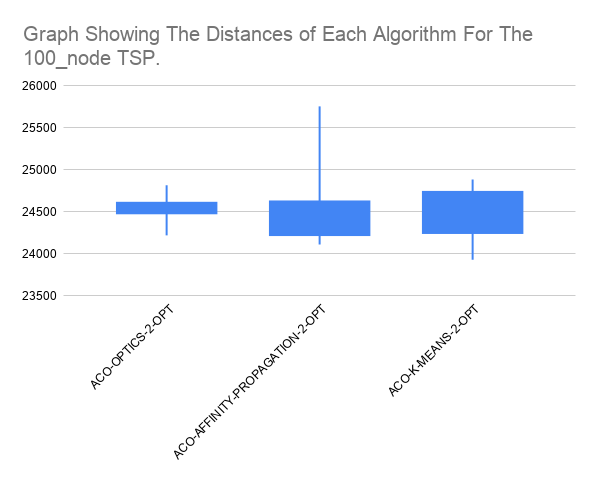
\includegraphics[width=\textwidth]{figures/tsp_distance_100_node_graph.png}
    \caption{Box plot which shows the distances that were achieved when running the algorithms over the 100\_node TSP.}
    \label{fig:tsp_distance_100_node_graph}
\end{figure}

\begin{figure}
    \centering
    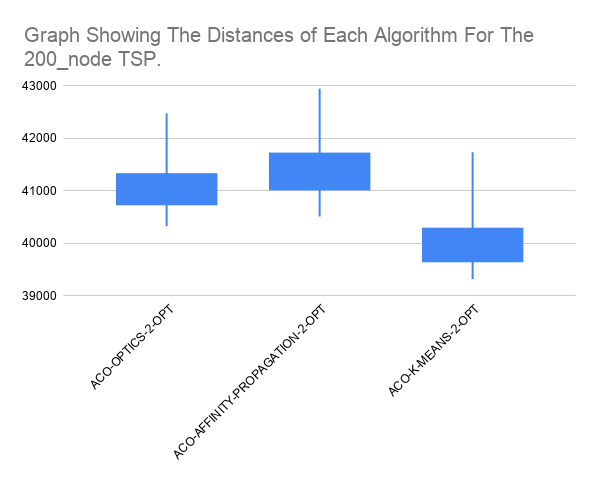
\includegraphics[width=\textwidth]{figures/tsp_distance_200_node_graph.png}
    \caption{Box plot which shows the distances that were achieved when running the algorithms over the 200\_node TSP.}
    \label{fig:tsp_distance_200_node_graph}
\end{figure}

\begin{figure}
    \centering
    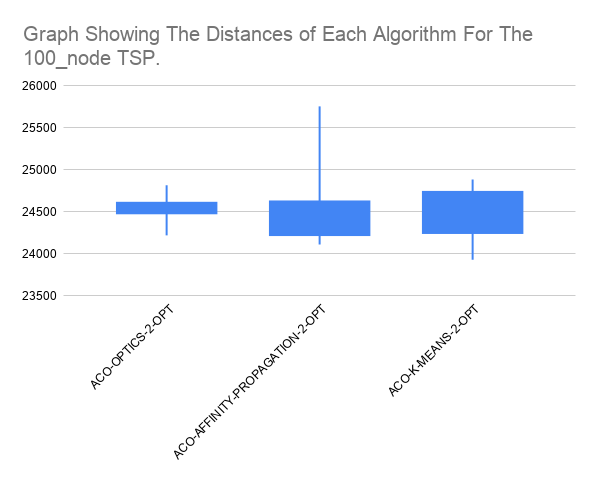
\includegraphics[width=\textwidth]{figures/tsp_distance_100_node_graph.png}
    \caption{Box plot which shows the distances that were achieved when running the algorithms over the 300\_node TSP.}
    \label{fig:tsp_distance_300_node_graph}
\end{figure}

\begin{figure}
    \centering
    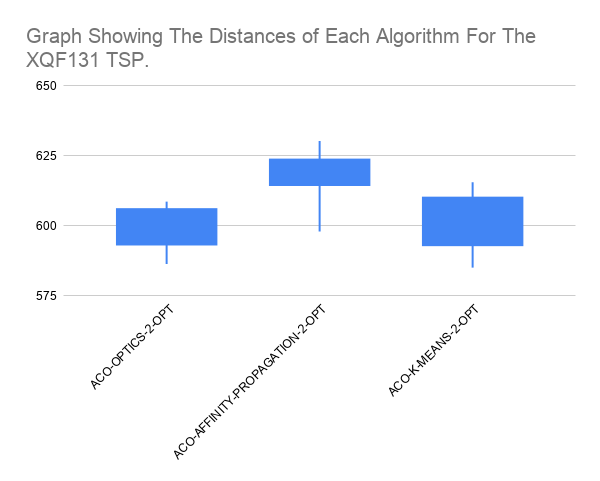
\includegraphics[width=\textwidth]{figures/tsp_distance_xqf131_graph.png}
    \caption{Box plot which shows the distances that were achieved when running the algorithms over the XQF TSP.}
    \label{fig:tsp_distance_xqf131_graph}
\end{figure}

\begin{figure}
    \centering
    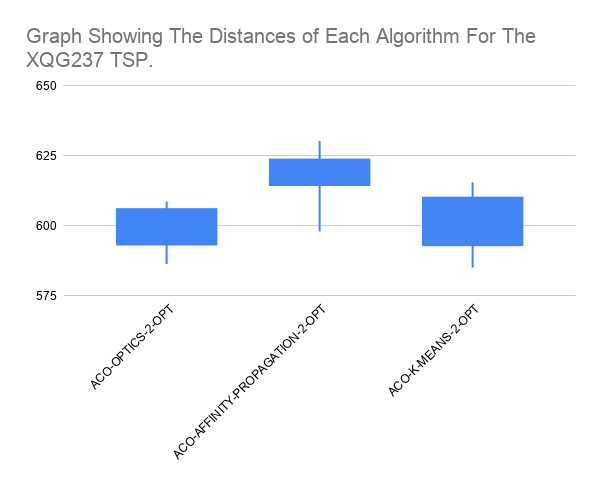
\includegraphics[width=\textwidth]{figures/tsp_distance_xqg237_graph.png}
    \caption{Box plot which shows the distances that were achieved when running the algorithms over the XGQ237 TSP.}
    \label{fig:tsp_distance_xqg237_graph}
\end{figure}

\begin{figure}
    \centering
    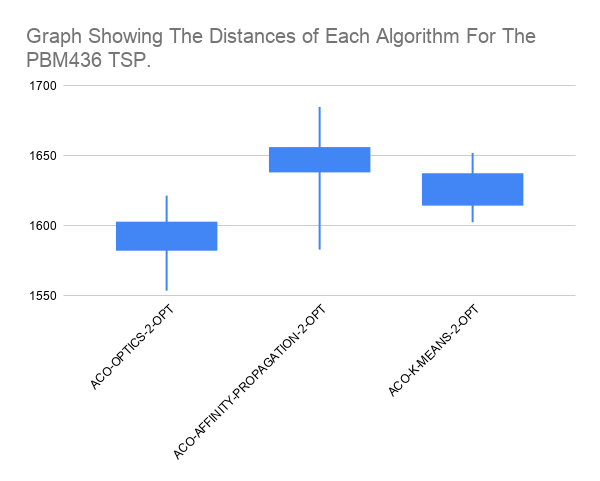
\includegraphics[width=\textwidth]{figures/tsp_distance_pbm436_graph.png}
    \caption{Box plot which shows the distances that were achieved when running the algorithms over the PBM436 TSP.}
    \label{fig:tsp_distance_pbm436_graph}
\end{figure}

Figures \ref{fig:tsp_distance_100_node_graph},  \ref{fig:tsp_distance_200_node_graph},  \ref{fig:tsp_distance_300_node_graph},  \ref{fig:tsp_distance_xqf131_graph},  \ref{fig:tsp_distance_xqg237_graph} and  \ref{fig:tsp_distance_pbm436_graph} show the distances that were achieved for these algorithms.

Comparing these set of graphs to the non 2-opt runs which were presented in section \ref{sec:question2} they show a large improvement. The graphs show a lot less variation and the distances produced are much more consistent amongst the algorithms. 

2-opt is a local search algorithm and therefore will only find the locally optimal solution based on the tour that was passed into it. It is always looking for an improvement and won't make a change to the tour unless it results in a lower tour length, for some tours it will be necessary to make the tour worse in order for an improvement to be found. In order to cut down on the run time it doesn't make these kind of changes. 

The OPTICS run for the 300\_node TSP is interesting because it is much better than the others, the OPTICS run for this problem generates 20 clusters 103 noisy nodes that it can't cluster. This means that the initial ACO run is over 123 nodes, this leads me to believe that structures that the data fall into are very similar amongst all the clustering algorithms and 2-opt finds the optimal version of the tour in this structure. However when you have an algorithm like OPTICS which doesn't put every node into a cluster you end up not falling into that structure and therefore the locally optimal solution that 2-opt finds is different and in this case improved.

VLSI data shows similar results, the tour lengths are closer to each other so the clustering algorithms all return similar clusters that have the same optimal solutions. OPTICS performs better than other algorithms with VLSI data as well, as I've discussed earlier OPTICS performs badly when clustering VLSI data and the same points are true here as well. OPTICS can't cluster the strcutres that are present in VLSI data, it wants to cluster circularly but as VLSI data consists of lines it can't cluster this, and therefore the locally optimal tour that 2-opt finds is the tour that was created by ACO running over lots of nodes.

Affinity Propagation and K-Means give very similar results when 2-opt is ran. The variances of the data are similar as are the average values. It would make sense that these two clustering algorithms give similar results because they work in very similar ways except that Affinity Propagation estimates the number of nodes that are in the data. As both of these algorithms put every node into a cluster it seems that the data and the structure of this data is very similar even though they both produce different numbers of clusters.

These results were not what I was expecting, I assumed that the clusters that were generated would be different enough for the optimal tour that 2-opt found to be significantly different but this turned out to not be the case.

\section{What effect does varying the ACO parameters have on the solution?}

This question was about seeing if there were optimal parameters that could be set on ACO when running with a clustering algorithm. To test this I chose one TSP problem and one clustering algorithm and then varied the parameters to see the effects on both run time and the distance of the tour. When I was testing the parameters I only changed one parameter at a time, the base set of parameters I used was: 300 iterations, number of ants is number of nodes divided by 1.5, $\alpha$ is 1, $\beta$ is 10, $\rho$ is 0.4 and $Q$ is 1000. The K-Means k value was 20. As with all the other experiments I run this ten times as well. I chose the 200\_node problem to run this on because I thought that it was large enough for the changes to be noticeable but small enough for the runs to not take too long.

I varied the alpha, beta, rho, q and ant count values, for each parameter I tested three values. For alpha I set the values to 0.5, 1 and 1.5, for beta I set the values to 5, 10 and 15, for q I set the values to 500, 1000, 1500, for rho I set the values to 0.2, 0.4 and 1 and I set the ant count to 133, 200 and 400. I chose these values for the ant count because it was the number of nodes in the TSP divided by 1.5, the number of nodes in the TSP and the number of nodes in the TSP multiplied by 2.

\begin{longtable}[c]{|l|l|l|}
\hline
\multicolumn{3}{|c|}{Alpha Value} \\ \hline
\endhead
%
     & Distance     & Run Time    \\ \hline
0.5  & 45609.3870   & 180.5890    \\ \hline
1    & 45733.7063   & 165.4209   \\ \hline
1.5  & 46122.7783  & 180.5890 \\ \hline
\caption{This table shows the average run times and tour lengths when the alpha values were varied.}
\label{tab:alpha_aco_table}\\
\end{longtable}

\begin{longtable}[c]{|l|l|l|}
\hline
\multicolumn{3}{|c|}{Ant Count}  \\ \hline
\endfirsthead
%
\endhead
%
    & Distance    & Run Time   \\ \hline
133 & 45733.7063 & 165.4208  \\ \hline
200 & 45398.0928 & 223.1873 \\ \hline
400 & 45441.4907 & 431.1539 \\ \hline
\caption{This table shows the run times and tour lengths when the ACO ant count were varied. Here the number of ants was varied so that it was the number of nodes/1.5, the number of nodes and the number of nodes * 2.}
\label{tab:ant_count_aco_table}\\
\end{longtable}

\begin{longtable}[c]{|l|l|l|}
\hline
\multicolumn{3}{|c|}{Beta}     \\ \hline
\endfirsthead
%
\endhead
%
   & Distance    & Run Time  \\ \hline
5  & 45505.8459 & 177.9760   \\ \hline
10 & 45733.7063 & 165.4209   \\ \hline
15 & 45788.4176 & 154.8633 \\ \hline
\caption{This table shows the the run time and tour length when varying the beta value.}
\label{tab:beta_aco_table}\\
\end{longtable}

\begin{longtable}[c]{|l|l|l|}
\hline
\multicolumn{3}{|c|}{Q}      \\ \hline
\endfirsthead
%
\endhead
%
     & Distance   & Run Time \\ \hline
500  & 45505.8459 & 177.9760 \\ \hline
1000 & 45733.7063 & 165.4209 \\ \hline
1500 & 45788.4176 & 154.8633 \\ \hline
\caption{This table shows the run times and tour lengths when varying the Q ACO parameter.}
\label{tab:q_aco_table}\\
\end{longtable}

\begin{longtable}[c]{|l|l|l|}
\hline
\multicolumn{3}{|c|}{Rho}    \\ \hline
\endfirsthead
%
\endhead
%
     & Distance   & Run Time \\ \hline
500  & 45505.8459 & 177.9760 \\ \hline
1000 & 45733.7063 & 165.4209 \\ \hline
1500 & 45788.4176 & 154.8633 \\ \hline
\caption{This table shows the run times and lengths when varying the rho ACO parameter.}
\label{tab:rho_aco_table}\\
\end{longtable}

Tables \ref{tab:ant_count_aco_table}, \ref{tab:q_aco_table}, \ref{tab:rho_aco_table}, \ref{tab:beta_aco_table} and \ref{tab:alpha_aco_table} show the results of varying these parameters. 

These results don't show a huge difference the tour lengths are very similar amongst all the parameters. There are a few differences that can be mentioned. The lower Q value improves the length of the tour, Q affects how much pheromone gets deposited. This means that the ants are more likely to choose a new path because the scent isn't as strong. This could just be random chance though because even though I've run this ten times ACO still has elements of randomness so these could just be good runs and the ants have randomly chosen good pathways.

Increasing the number of ants increases the run time quite a lot, this does make sense though because the more ants there are to simulate the more times the algorithm has to run so the longer it will take. As shown in Chapter 1 the run time of ACO is proportional to the number of ants.

This question might have not been broad enough and not run the right sets of parameters. Instead of changing one parameter it might have been better to change many parameters at one time, in \cite{gaertner_clark} they attempted to find the optimal ACO parameters and changed three parameters: beta, rho and \[q_{0}\]. They varied each of these parameters and ran the test ten times for each combination this resulted in 13,860 runs. This did get them a result though and they did identify optimal values, this is a question that could be explored further in the future. 
\chapter{Evaluation}

In my project I have shown that the performance of ACO can be improved through the use of a clustering algorithm and gone some way to find what that clustering algorithm should be. I have also shown the poor performance of clustering algorithms on complex VLSI data and how 2-opt can help improve upon tours and how the clustering algorithms all return data in a similar structure which allows 2-opt to find similar tours amongst all clustering algorithms.

\section{Process}

I adopted a version of Scrum I followed it reasonably closely and the use of Jira definitely helped. I found weekly sprints to be a really good way of planning my next week, however sometimes I didn't follow them all that closely or I let the sprints take slightly longer than a week. I could have followed this process more closer. 

I implemented all the requirements that were needed to run my tests and there was only one feature that I would have liked to implement but ran out of time to do so. This was an improved clustering algorithm. This was always an extension feature but if I had focused more on it and given it a higher priority then I might have been able to do it. 

\section{Implementation}

I'm happy with my code and my implementation I feel that I made a good choice using Python even though it's quite a slow language to run it is easy to write and comes with lots of useful features and libraries which sped up the implementation phase of my project.

The run time of the experiments was a big problem and if I had chosen C++ then this would have been less of an issue. C++ is a much faster language and would have allowed me to run more experiments and investigate more questions.

The code was quite inefficient in places there are areas that would really benefit from multi threading such as ACO and 2-OPT. I did implement a second ACO library that used multi threading but I never used it in any tests because it generated tours which were worse than those generated by ACOPY.

\subsection{Testing}
 
There was not very much testing, I did make up for this with my own manual testing but this was not controlled; there was no test table I just ran through the program and ensured it worked, but there was no procedure for how to do this. I should have implemented more unit tests that covered everything in the project. I did unit test some areas but I felt that unit testing the entire project would be too complex and take too a long time, maybe this is true but it would have given me more confidence in my code and allow for errors in my code to be spotted more quickly.

\section{Experiments}

I'm mostly pleased with the results I achieved in my experiments however there were a few problems.

I didn't anticipate how long these experiments would take to run especially for the larger problems. It ended up taking 345 hours to run all the tests which was much longer than I had planned. Most of this time was spent running the larger problems and I could have saved a considerable amount of time if I had chosen smaller sized problems.

I also didn't want to use my computer when I was running these tests in case my use negatively impacted the run time of the algorithms so I couldn't do work on my report. If I had access to another computer then I could have left my computer running these tests and worked on my report, due to the current circumstances and not being able to use any University facilities this was not possible.

The experiment looking into ACO parameters didn't show any significant results, if I had varied more parameters at one time then this would not have been a problem. I didn't have time to do this in my project especially towards the end, if I had spent less time running tests on larger problem files then I might have had time to run more experiments and could have potentially answered this question more thoroughly.

I could have been more efficient with my experiments and carried them out in a more automated way. When I ran the experiments I had to then then had to go through the log files to extract the run time and distance information. This slowed down the process and was a very tedious task. I also did the 2-opt runs separate to the non 2-opt runs which slowed me down and duplicated a lot of the work I had to do, what I should have done instead, is have those run once and then record the time taken and tour lengths before and after 2-opt.

\section{Future Work}

This project is very broad and covers lots of areas of Computer Science, this means that there were features I would have liked to implement and experiments I would have liked to run but couldn't due to the short nature of this project.

It would have been interesting to look at what the optimal K-Means value is for a piece of data. As I have shown K-Means is sometimes the best performing clustering algorithm however it needs a k value so it knows how many clusters to create in the data. This k value may be related to the size of the data, if several k values were chosen for several pieces of data then a pattern may emerge and you may be able to show what the optimal.

There are other clustering algorithms that I didn't experiment with, it may be possible that one of these performs better with TSP data or one of these is better suited to VLSI data. My experiments showed that VLSI data is very tricky to cluster and all the algorithms that I have implemented do quite a poor job. There may be an already created clustering algorithm that performs really well on this type of data.

The experiment where I tested optimal ACO values didn't yield any significant results. This was down to the tests only changing one parameter at a time and ACO is dependent on many parameters it would be nice to re-do this experiment and change many parameters at one time, this would take a long time to run and would be thousands of ACO runs.

One of the things I wanted to do but didn't have enough time for was to create a new clustering algorithm that expands to fit the complex data present in TSPs. This would be similar to the algorithm developed in \cite{pang_chao-yang_ben-qiong_zhang_jie_wei_shan_zheng-chao_2014}, it would map out the expansions of data and then cluster to fit those expansions. This should result in shorter tours that are found quicker but required a lot of work that I didn't have time for.

There are versions of 2-opt that swap more nodes and might find higher quality tours. 2.5-opt and 3-opt it would be interesting to see their effects on the tours and see how much they can improve it. Although there still only perform local searches so the improvements they can make are limited and they are unlikely to find the globally optimal solution. 

I implemented a greedy nearest neighbours search algorithm to calculate the tours in every cluster, however I never used this in my experiments. It would be interesting to compare this against ACO for in cluster tour generation.

I implemented the BIRCH clustering algorithm but never used it in any tests because you need to choose several parameters. In the future the impact of BIRCH on TSPs could be explored, BIRCH performs well with lots of nodes so could potentially improve the tours of the large TSPs. 

\section{What I Would Do Differently}

If I was to redo this project I would give myself longer to run the experiments as this was in my opinion the biggest failure in my project. If I had started running experiments earlier or had access to more computers then this would not of been a big problem. I would also run the experiments on smaller problems instead of choosing 100, 200 and 300 node problems I should have chosen 100, 150 and 200 node problems, the larger problems took too long to run and could have benefited from the ACO being run for more iterations.

I would have also spent more time focusing on the better clustering algorithm, this is a feature that would result in a big improvement in tours and a reduction in run time. I would focus a much greater proportion of time on this feature.

% add any additional chapters here

%TC:ignore
\setemptyheader

\nocite{*} % include everything from the bibliography, irrespective of whether it has been referenced.

% the following line is included so that the bibliography is also shown in the table of contents. There is the possibility that this is added to the previous page for the bibliography. To address this, a newline is added so that it appears on the first page for the bibliography. 
\addcontentsline{toc}{chapter}{Annotated Bibliography} % Adds References to contents page

%
% example of including an annotated bibliography. The current style is an author date one. If you want to change, comment out the line and uncomment the subsequent line. You should also modify the packages included at the top (see the notes earlier in the file) and then trash your aux files and re-run. 
%\bibliographystyle{StylesAndReferences/authordate2annot}
\bibliographystyle{StylesAndReferences/IEEEannotU}
\renewcommand{\bibname}{Annotated Bibliography} 

\bibliography{StylesAndReferences/references} % References file


\setemptyheader

\addcontentsline{toc}{chapter}{Appendices}
\chapter*{Appendices}
The appendices are for additional content that is useful to support the discussion in the report. It is material that is not necessarily needed in the body of the report, but its inclusion in the appendices makes it easy to access. 

For example, if you have developed a Design Specification document as part of a plan-driven approach for the project, then it would be appropriate to include that document as an appendix. In the body of your report you would highlight the most interesting aspects of the design, referring your reader to the full specification for further detail.

If you have taken an agile approach to developing the project, then you may be less likely to have developed a full requirements specification. Perhaps you use stories to keep track of the functionality and the 'future conversations'. It might not be relevant to include all of those in the body of your report. Instead, you might include those in an appendix. 

There is a balance to be struck between what is relevant to include in the body of your report and whether additional supporting evidence is appropriate in the appendices. Speak to your supervisor or the module coordinator if you have questions about this.

\pagebreak

% start the appendix - sets up different numbering
\fancypagestyle{plain}{%
%\fancyhf{} % clear all header and footer fields
\fancyhead[L]{Appendix\ \thechapter}
\fancyhead[R]{\leftmark}}

\appendix
\fancyhead[L]{Appendix\ \thechapter}
\fancyhead[R]{\leftmark}
\fancyhead[C]{}
\fancyfoot[C]{\thepage}
\renewcommand{\headrulewidth}{0.4pt}
\renewcommand{\chaptermark}[1]{\markboth{#1}{}}

\fancyhead[L]{Appendix\ \thechapter}
\fancyhead[R]{\leftmark}
\fancyfoot[C]{{\thepage} of \pageref{LastPage}}

% include any appendices here
\chapter{Third-Party Code and Libraries}

If you have made use of any third party code or software libraries, i.e. any code that you have not designed and written yourself, then you must include this appendix. 

As has been said in lectures, it is acceptable and likely that you will make use of third-party code and software libraries. If third party code or libraries are used, your work will build on that to produce notable new work. The key requirement is that we understand what your original work is and what work is based on that of other people. 

Therefore, you need to clearly state what you have used and where the original material can be found. Also, if you have made any changes to the original versions, you must explain what you have changed. 

The following is an example of what you might say. 

Apache POI library - The project has been used to read and write Microsoft Excel files (XLS) as part of the interaction with the client's existing system for processing data. Version 3.10-FINAL was used. The library is open source and it is available from the Apache Software Foundation 

Include as many declarations as appropriate for your work. The specific wording is less important than the fact that you are declaring the relevant work.
\chapter{Ethics Submission}

This appendix includes a copy of the ethics submission for the project. After you have completed your Ethics submission, you will receive a PDF with a summary of the comments. That document should be embedded in this report, either as images, an embedded PDF or as copied text. The content should also include the Ethics Application Number that you receive. 
\chapter{List of Requirements}\label{appendix_requirements}

These are the requirements that my project must fulfill in order for me to carry out my experiments as required.

\begin{itemize}
    \item Load in TSP files.
        \begin{itemize}
            \item Needs to be able to load in common TSPLIB files.
            \item Have the data available as an Array.
            \item Have the data available as a graph.
            \item Plot a graph showing all the nodes.
        \end{itemize}
    \item Perform clustering.
        \begin{itemize}
            \item Implement the Birch clustering algorithm.
            \item Implement the K-Means clustering algorithm.
            \item Implement the DBSCAN clustering algorithm.
            \item Implement the Affinity Propagation clustering algorithm.
            \item Implement the OPTICS clustering algorithm.
            \item Automate a version of the DBSCAN algorithm that finds the eps value itself.
            \item All the clustering algorithms should output the clusters in a common format and data structure.
            \item Plot a graph showing all the clusters.
            \item Attempt to implement a new clustering algorithm that can better deal with TSP data.
            \begin{itemize}
                \item This does not necessarily have to be done it would just be interesting to see if this is possible although given the time available it may not be possible.
            \end{itemize}
        \end{itemize}
    \item Carry out ACO.
        \begin{itemize}
            \item Find an ACO library or implement my own.
            \item Plot a graph of the ACO tour.
            \item Visualise the incremental improvements that ACO makes.
                \begin{itemize}
                    \item It would be nice to have a GIF or a video that shows all the iterations that ACO went through to reach the final ACO tour.
                \end{itemize}
        \end{itemize}
    \item 2-opt.
        \begin{itemize}
            \item Implement 2-opt.
            \item Visualise the improvement that 2-opt makes.
                \begin{itemize}
                    \item It would be nice to see the incremental improvements that 2-opt makes when it finds a node to swap and reach a lower tour length. This could be as a GIF or a video, this can reuse the code that was written for the 'Visualise the incremental improvements that ACO makes' above.
                \end{itemize}
        \end{itemize}
    \item Have a way to go from the tour of the global tour of the clusters to a tour through each cluster.
        \begin{itemize}
            \item Find the two closest nodes between each cluster of the tour.
            \item For each cluster record the nodes that are the entry/exit nodes.
        \end{itemize}
    \item Tour inside clusters.
        \begin{itemize}
            \item Calculate the tour inside each cluster using ACO.
            \item Calculate the tour inside each cluster using a greedy nearest neighbours. approach
            \item These tours have to start from the entry node and work towards the exit node.
            \item Plot a graph of each cluster showing the tour.
        \end{itemize}
    \item Validate the tour.
        \begin{itemize}
            \item Ensure the tour travels over every node.
            \item Ensure the tour doesn't visit any node twice.
        \end{itemize}
    \item Record the time taken for the program to run.
        \begin{itemize}
            \item The time taken for 2-opt should be recorded separately.
            \item The time taken for graphs to be generated shouldn't be recorded.
        \end{itemize}
    \item Calculate the length of the tour.
        \begin{itemize}
            \item Calculate this before and after 2-opt is run.
        \end{itemize}
\end{itemize}

\fancypagestyle{plain}{%
   \fancyhead{} %[C]{Annotated Bibliography}
   \fancyfoot[C]{{\thepage} of \pageref{LastPage}} % except the center
   \renewcommand{\headrulewidth}{0pt}
   \renewcommand{\footrulewidth}{0pt}
}

%TC:endignore

\end{document}
